% This is a template for Ph.D. dissertations in the UCI format.
%
% All fonts, including those for sub- and superscripts, must be 10
% points or larger.  Recommended sizes are 14-point for chapter
% headings, 12-point for the main body of text and figure/table
% titles, and 10-point for footnotes, sub- and super-scripts, and text
% in figures and tables.
%
% Notes: Add short title to figures, sections, via square brackets,
% e.g. \section[short]{long}.
%
\documentclass[12pt,fleqn]{ucithesis}

% A few common packages
\usepackage{amsmath}
\usepackage{amsthm}
\usepackage{array}
\usepackage{graphicx}
\usepackage{natbib}
\usepackage{relsize}

% Some other useful packages
\usepackage{caption}
\usepackage{multirow}
\usepackage{booktabs}
\usepackage{subfigure}
\usepackage{threeparttable}
\usepackage{xcolor} % provides \colorlet
\usepackage{fixme}

% fixme stuff
\fxsetup{
    status=draft,
    author=Wei,
    layout=inline,
    theme=color
}
\definecolor{fxnote}{rgb}{0.8000,0.0000,0.0000}
\colorlet{fxnotebg}{yellow}
% refedine the layout macro:
\makeatletter
\renewcommand*\FXLayoutInline[3]{%
  \@fxdocolon {#3}{%
    \@fxuseface {inline}%
    \colorbox{fx#1bg}{\color {fx#1}\ignorespaces #3\@fxcolon #2}}}
\makeatother

% plainpages=false fixes the "duplicate ignored" error with page counters
% Set pdfborder to 0 0 0 to disable colored borders around PDF hyperlinks
\usepackage[plainpages=false,pdfborder={0 0 0}]{hyperref}

% Uncomment the following two lines to use the algorithm package,
% which provides an algorithm environment similar to figure and table
% ("\begin{algorithm}...\end{algorithm}"). A list of algorithms will
% automatically be added in the preliminary pages. Note that you
% probably want a package for the actual code to go with this (e.g.,
% algorithmic).
%\usepackage{algorithm}
%\renewcommand{\listalgorithmname}{\protect\centering\protect\Large LIST OF ALGORITHMS}

% Uncomment the following line to enable Unicode support. This will allow you
% to enter non-ASCII characters (such as accented characters) directly without
% having to use LaTeX's awkward escape syntax (e.g., \'{e})
% NOTE: You may have to install the ucs.sty package for this to work. See:
% http://www.unruh.de/DniQ/latex/unicode/
%\usepackage[utf8x]{inputenc}

% Uncomment the following to avoid "widowing", where page breaks cause
% single lines of paragraphs to float onto the next page (this is not
% a UCI requirement but more of an aesthetic choice).
%\widowpenalty=10000
%\clubpenalty=10000

% Modify or extend these at will.
\newtheorem{theorem}{\textsc{Theorem}}[chapter]
\newtheorem{definition}{\textsc{Definition}}[chapter]
\newtheorem{example}{\textsc{Example}}[chapter]

% Benchmarking numbers
\newcommand{\zippyToCPythonRegular}{15.34}

\newcommand{\peelingSpeedup}{3.58}
\newcommand{\zippyToCPython}{20.59}
\newcommand{\pypyToCPython}{10.53}

% Macros for title, author, abstract, etc.
\thesistitle{Efficient Hosted Interpreter for Dynamic Languages}

\degreename{Doctor of Philosophy}

% Use the wording given in the official list of degrees awarded by UCI:
% http://www.rgs.uci.edu/grad/academic/degrees_offered.htm
\degreefield{Computer Engineering}

% Your name as it appears on official UCI records.
\authorname{Wei Zhang}

% Use the full name of each committee member.
\committeechair{Professor Michael Franz}
\othercommitteemembers
{
  Professor Kwei-Jay Lin\\
  Professor Guoqing Xu
}

\degreeyear{2015}

\copyrightdeclaration
{
  Portion of Chapter~\ref{chp:ch3-bytecode} {\copyright} $2013$, $2014$ ACM \\
  Portion of Chapter~\ref{chp:ch4-zippy} {\copyright} $2014$ ACM \\
  Portion of Chapter~\ref{chp:ch5-peeling} {\copyright} $2014$ ACM \\
  All other materials {\copyright} {\Degreeyear} \Authorname
}

% If you have previously published parts of your manuscript, you must list the
% copyright holders; see Section 3.2 of the UCI Thesis and Dissertation Manual.
% Otherwise, this section may be omitted.
% \prepublishedcopyrightdeclaration
% {
% 	Chapter 4 {\copyright} 2003 Springer-Verlag \\
% 	Portion of Chapter 5 {\copyright} 1999 John Wiley \& Sons, Inc. \\
% 	All other materials {\copyright} {\Degreeyear} \Authorname
% }

% The dedication page is optional.
\dedications
{

  To my supporting parents and lovely wife.
}

\acknowledgments
{
  First and foremost, I would like to thank my advisor Professor Michael Franz for his mentorship and support during my years in graduate school.
  I am deeply grateful that he admitted me to his fantastic research group and brought me into the world of programming languages.
  Working under his supervision has been one of my most fulfilling period of my life.

  I would also like to thank Professor Kwei-Jay Lin and Professor Guoqing Xu for accepting to serve on my committee.

  I am deeply grateful for Dr. Stefan Brunthaler and Dr. Per Larsen for closely working with me on this research.
  Their continuous guidance, motivation and insightful comments greatly improve me as a graduate student researcher.
  This thesis would not be possible without their help.

  I would also like to thank Dr. Christian Wimmer for his valuable feedback to my work and mentorship during my internships at Oracle Labs.
  I am also grateful to Chris Seaton, Andreas Woess and other people I have worked with at Oracle Labs.
  Their mastery on software design deeply inspired me.

  Lastly, I would like to thank my amazing colleagues.
  I have been fortunate to be a part of this great research group.
  My thanks go to: Mason Chang, Todd Jackson, Michael Bebenita, Christoph Kerschbaumer, Gregor Wagner, Eric Hennigan, 
  Andrei Homescu, G{\"u}lfem Savrun-Yeniçeri, Stephen Crane, Mark Murphy, Codru\c{t} Stancu, Mohaned Qunaibit, Brian Belleville and Julian Lettner.
}


% Some custom commands for your list of publications and software.
\newcommand{\mypubentry}[3]{
  \begin{tabular*}{1\textwidth}{@{\extracolsep{\fill}}p{4.5in}r}
    \textbf{#1} & \textbf{#2} \\
    \multicolumn{2}{@{\extracolsep{\fill}}p{.95\textwidth}}{#3}\vspace{6pt} \\
  \end{tabular*}
}
\newcommand{\mysoftentry}[3]{
  \begin{tabular*}{1\textwidth}{@{\extracolsep{\fill}}lr}
    \textbf{#1} & \url{#2} \\
    \multicolumn{2}{@{\extracolsep{\fill}}p{.95\textwidth}}
    {\emph{#3}}\vspace{-6pt} \\
  \end{tabular*}
}

% Include, at minimum, a listing of your degrees and educational
% achievements with dates and the school where the degrees were
% earned. This should include the degree currently being
% attained. Other than that it's mostly up to you what to include here
% and how to format it, below is just an example.
\curriculumvitae
{

\textbf{EDUCATION}

  \begin{tabular*}{1\textwidth}{@{\extracolsep{\fill}}lr}
    \textbf{Doctor of Philosophy in Computer Engineering} & \textbf{2015} \\
    \vspace{6pt}
    University of California, Irvine & \emph{Irvine, California} \\

    \textbf{Master of Science in Computer Engineering} & \textbf{2010} \\
    \vspace{6pt}
    Chalmers University of Technology & \emph{Gothenburg, Sweden} \\

    \textbf{Bachelor of Science in Mechanical Engineering} & \textbf{2004} \\
    \vspace{6pt}
    University of Science and Technology Beijing & \emph{Beijing, China} \\
  \end{tabular*}

\vspace{12pt}
\textbf{RESEARCH EXPERIENCE}

  \begin{tabular*}{1\textwidth}{@{\extracolsep{\fill}}lr}
    \textbf{Graduate Student Researcher} & \textbf{2010--2015} \\
    \vspace{6pt}
    University of California, Irvine & \emph{Irvine, California} \\

    \textbf{Master Student Researcher} & \textbf{2010} \\
    \vspace{6pt}
    Chalmers University of Technology & \emph{Gothenburg, Sweden} \\
  \end{tabular*}

\vspace{12pt}
\textbf{PROFESSIONAL EXPERIENCE}

  \begin{tabular*}{1\textwidth}{@{\extracolsep{\fill}}lr}
    \textbf{Software Development Intern} & \textbf{Summer 2014} \\
    \vspace{6pt}
    Oracle Labs & \emph{Belmont, CA} \\

    \textbf{Software Development Intern} & \textbf{Summer 2013} \\
    \vspace{6pt}
    Oracle Labs & \emph{Belmont, CA} \\

    \textbf{Customer Service Engineer} & \textbf{2007--2008} \\
    \vspace{6pt}
    ASML & \emph{Shanghai, China} \\

    \textbf{Production Engineer} & \textbf{2005--2007} \\
    \vspace{6pt}
    AT\&S & \emph{Shanghai, China} \\

    \textbf{Mechanical Design Engineer} & \textbf{2004--2005} \\
    \vspace{6pt}
    BMEI & \emph{Beijing, China} \\
  \end{tabular*}

\pagebreak

\textbf{PUBLICATIONS}

  % \mypubentry{Awesome paper}{Jun 2011}{Conference name}
  % \mypubentry{Another awesome paper}{Aug 2012}{Conference name}

Wei Zhang, Per Larsen, Stefan Brunthaler, Michael Franz.
\textbf{Accelerating Iterators in Optimizing AST Interpreters}.
\textit{In Proceedings of the 29th ACM SIGPLAN Conference on Object Oriented Programming:
Systems, Languages, and Applications, Portland, OR, USA, October 20-24, 2014 (OOPSLA '14)}, 2014.

G{\"u}lfem Savrun-Yeniçeri, Wei Zhang, Huahan Zhang, Eric Seckler, Chen Li, Stefan Brunthaler,
Per Larsen, Michael Franz.
\textbf{Efficient Hosted Interpreters on the JVM}.
\textit{In ACM Transactions on Architecture and Code Optimization, volume 11(1) pages 9:1–9:24}, 2014.

G{\"u}lfem Savrun-Yeniçeri, Wei Zhang, Huahan Zhang, Chen Li, Stefan Brunthaler, Per Larsen, Michael Franz.
\textbf{Efficient Interpreter Optimizations for the JVM}.
\textit{In Proceedings of the 10th International Conference on Principles and Practice of Programming in Java,
Stuttgart, Germany, September 11-13, 2013 (PPPJ '13)}, 2013.

\vspace{12pt}
\textbf{SOFTWARE}

\mysoftentry{ZipPy}{http://bitbucket.org/ssllab/zippy/}
{A fast and lightweight Python 3 implementation built using the Truffle framework.
It leverages the underlying Java JIT compiler and compiles Python programs to highly optimized machine code at runtime.}

\mysoftentry{ModularVM}{https://bitbucket.org/thezhangwei/modularvm/}
{An extension to the Maxine VM (Java Virtual Machine) that enables deeper integrations with JVM languages
like Jython (Python), Rhino (JavaScript) or JRuby (Ruby). It automatically accelerates guest language interpreters written in Java.}

}

% The abstract should not be over 350 words, although that's
% supposedly somewhat of a soft constraint.
\thesisabstract
{

Motivated by high development costs, production compilers and virtual machines, often support more than one language.
This strategy is most effective when the language family is homogeneous.
Many languages are very amenable to static program analysis, however, dynamic languages are not.
Consequently, a single VM cannot deliver peak performance for both types of languages without adapting its optimization strategy accordingly.

Informally, we host a ``highly dynamic'' language (Python) on the Java Virtual Machine, a VM for ``moderately dynamic'' languages.
While we are not the first to do so, our approach diverges from current practice by representing Python programs as abstract syntax trees, ASTs, rather than bytecode.
Not only are ASTs the simplest and most natural programming language implementation,
they also lend themselves well to optimizations those are particularly beneficial to highly dynamic languages.
Compared to Jython, which compiles Python programs to Java bytecode, our Python prototype is faster and requires less implementation effort.

}


%%% Local Variables: ***
%%% mode: latex ***
%%% TeX-master: "thesis.tex" ***
%%% End: ***


% Add PDF document info fields
\hypersetup{
	pdftitle={\Thesistitle},
	pdfauthor={\Authorname},
	pdfsubject={\Degreefield},
}

% Uncomment the following to have numbered subsubsections (by default
% numbering goes only to subsections).
%\setcounter{secnumdepth}{4}


% Set this to only select a subset of the includes directives below.
% Very handy to speed up compilation if you're working on a certain
% part of your thesis. It conserves page numbers, references, etc.
% even for non-included files.
%\includeonly{chapter1}

\begin{document}

% Preliminary pages are always loaded (TOC, CV, etc.)
\preliminarypages

% Include the different components of your thesis, in separate files.
% Using \include allows you to set \includeonly above.
\chapter{Introduction}

This is an example using the \LaTeX{} template for UCI theses and
dissertation documents \cite{uci-thesis-latex}. Figure
\ref{fig:sourcecode} is just for illustration purposes, as is Table
\ref{tab:coordinates}.

\begin{figure}
\begin{verbatim}
#include <iostream>
int main(int argc, char** argv) {
  std::cout << "Hello World." << std::endl;
  return 0;
}
\end{verbatim}
  \caption{Example source code.}
  \label{fig:sourcecode}
\end{figure}

\section{Background}

Lorem ipsum dolor sit amet, consectetur adipisicing elit, sed do
eiusmod tempor incididunt ut labore et dolore magna aliqua. Ut enim ad
minim veniam, quis nostrud exercitation ullamco laboris nisi ut
aliquip ex ea commodo consequat. Duis aute irure dolor in
reprehenderit in voluptate velit esse cillum dolore eu fugiat nulla
pariatur. Excepteur sint occaecat cupidatat non proident, sunt in
culpa qui officia deserunt mollit anim id est laborum.

\begin{table}
  \centering
  \begin{tabular}{|rr|r|}
    \hline
    $x$ & $y$ & $z$ \\
    \hline
    14 & 12 & -2 \\
    0 & 33 & -25 \\
    -3 & 11 & 22 \\
    4 & 4 & 6 \\
    \hline
  \end{tabular}
  \caption{Example coordinates.}
  \label{tab:coordinates}
\end{table}

Lorem ipsum dolor sit amet, consectetur adipisicing elit, sed do
eiusmod tempor incididunt ut labore et dolore magna aliqua. Ut enim ad
minim veniam, quis nostrud exercitation ullamco laboris nisi ut
aliquip ex ea commodo consequat. Duis aute irure dolor in
reprehenderit in voluptate velit esse cillum dolore eu fugiat nulla
pariatur. Excepteur sint occaecat cupidatat non proident, sunt in
culpa qui officia deserunt mollit anim id est laborum.


%%% Local Variables: ***
%%% mode: latex ***
%%% TeX-master: "thesis.tex" ***
%%% End: ***

\chapter{Hosted Bytecode Interpreter}

A programming language interpreter executes programs in two steps.
First it parses the human readable source code, verifies its correctness and translates the code into a more efficient intermediate representation (IR) format.
The interpreter then picks up the translated program and executes it piece by piece.

Bytecode interpreters parse source program into bytecode, a highly compressed representation of the program.
The format of the bytecode is a form of virtual instruction set designed for this particular interpreter.
In the second step bytecode interpreters execute the bytecode as a sequence of virtual instruction one instruction at a time before finishing the last one.
Interpreters are also regard as virtual machines, since they emulate ``machines'' with their own virtual instruction sets.

In this Chapter, we go over performance overheads of bytecode interpreters and the classic techniques used to minimize these overheads.
Lastly, we introduce ModularVM~\cite{savrun2013, savrun2014}, a research JVM that automatically optimize the performance of hosted bytecode interpreters.

\section{Performance Anatomy of Bytecode Interpreters}

Bytecode interpreters execute bytecode one instruction at a time.
For each instruction, the interpretation consists of three steps~\cite{davis2003case}:
\begin{itemize}
  \item Instruction dispatch
  \item Operand access
  \item Performing the function of the instruction
\end{itemize}
Instruction dispatch includes fetching the next instruction, decoding the instruction and transferring program execution to the actual implementation of the instruction.
Operand access involves fetching operands required to perform the instruction from either a temporal operand stack or a virtual register file depending on the design of the virtual instruction set.
It also includes storing the computed result back to where temporal operands should be stored.
Subsequently in the last step the interpreter performs the actual computation.
For instance, if the instruction is addition of two numbers, the actually addition is performed in this step.

\begin{figure}[th]
\centering
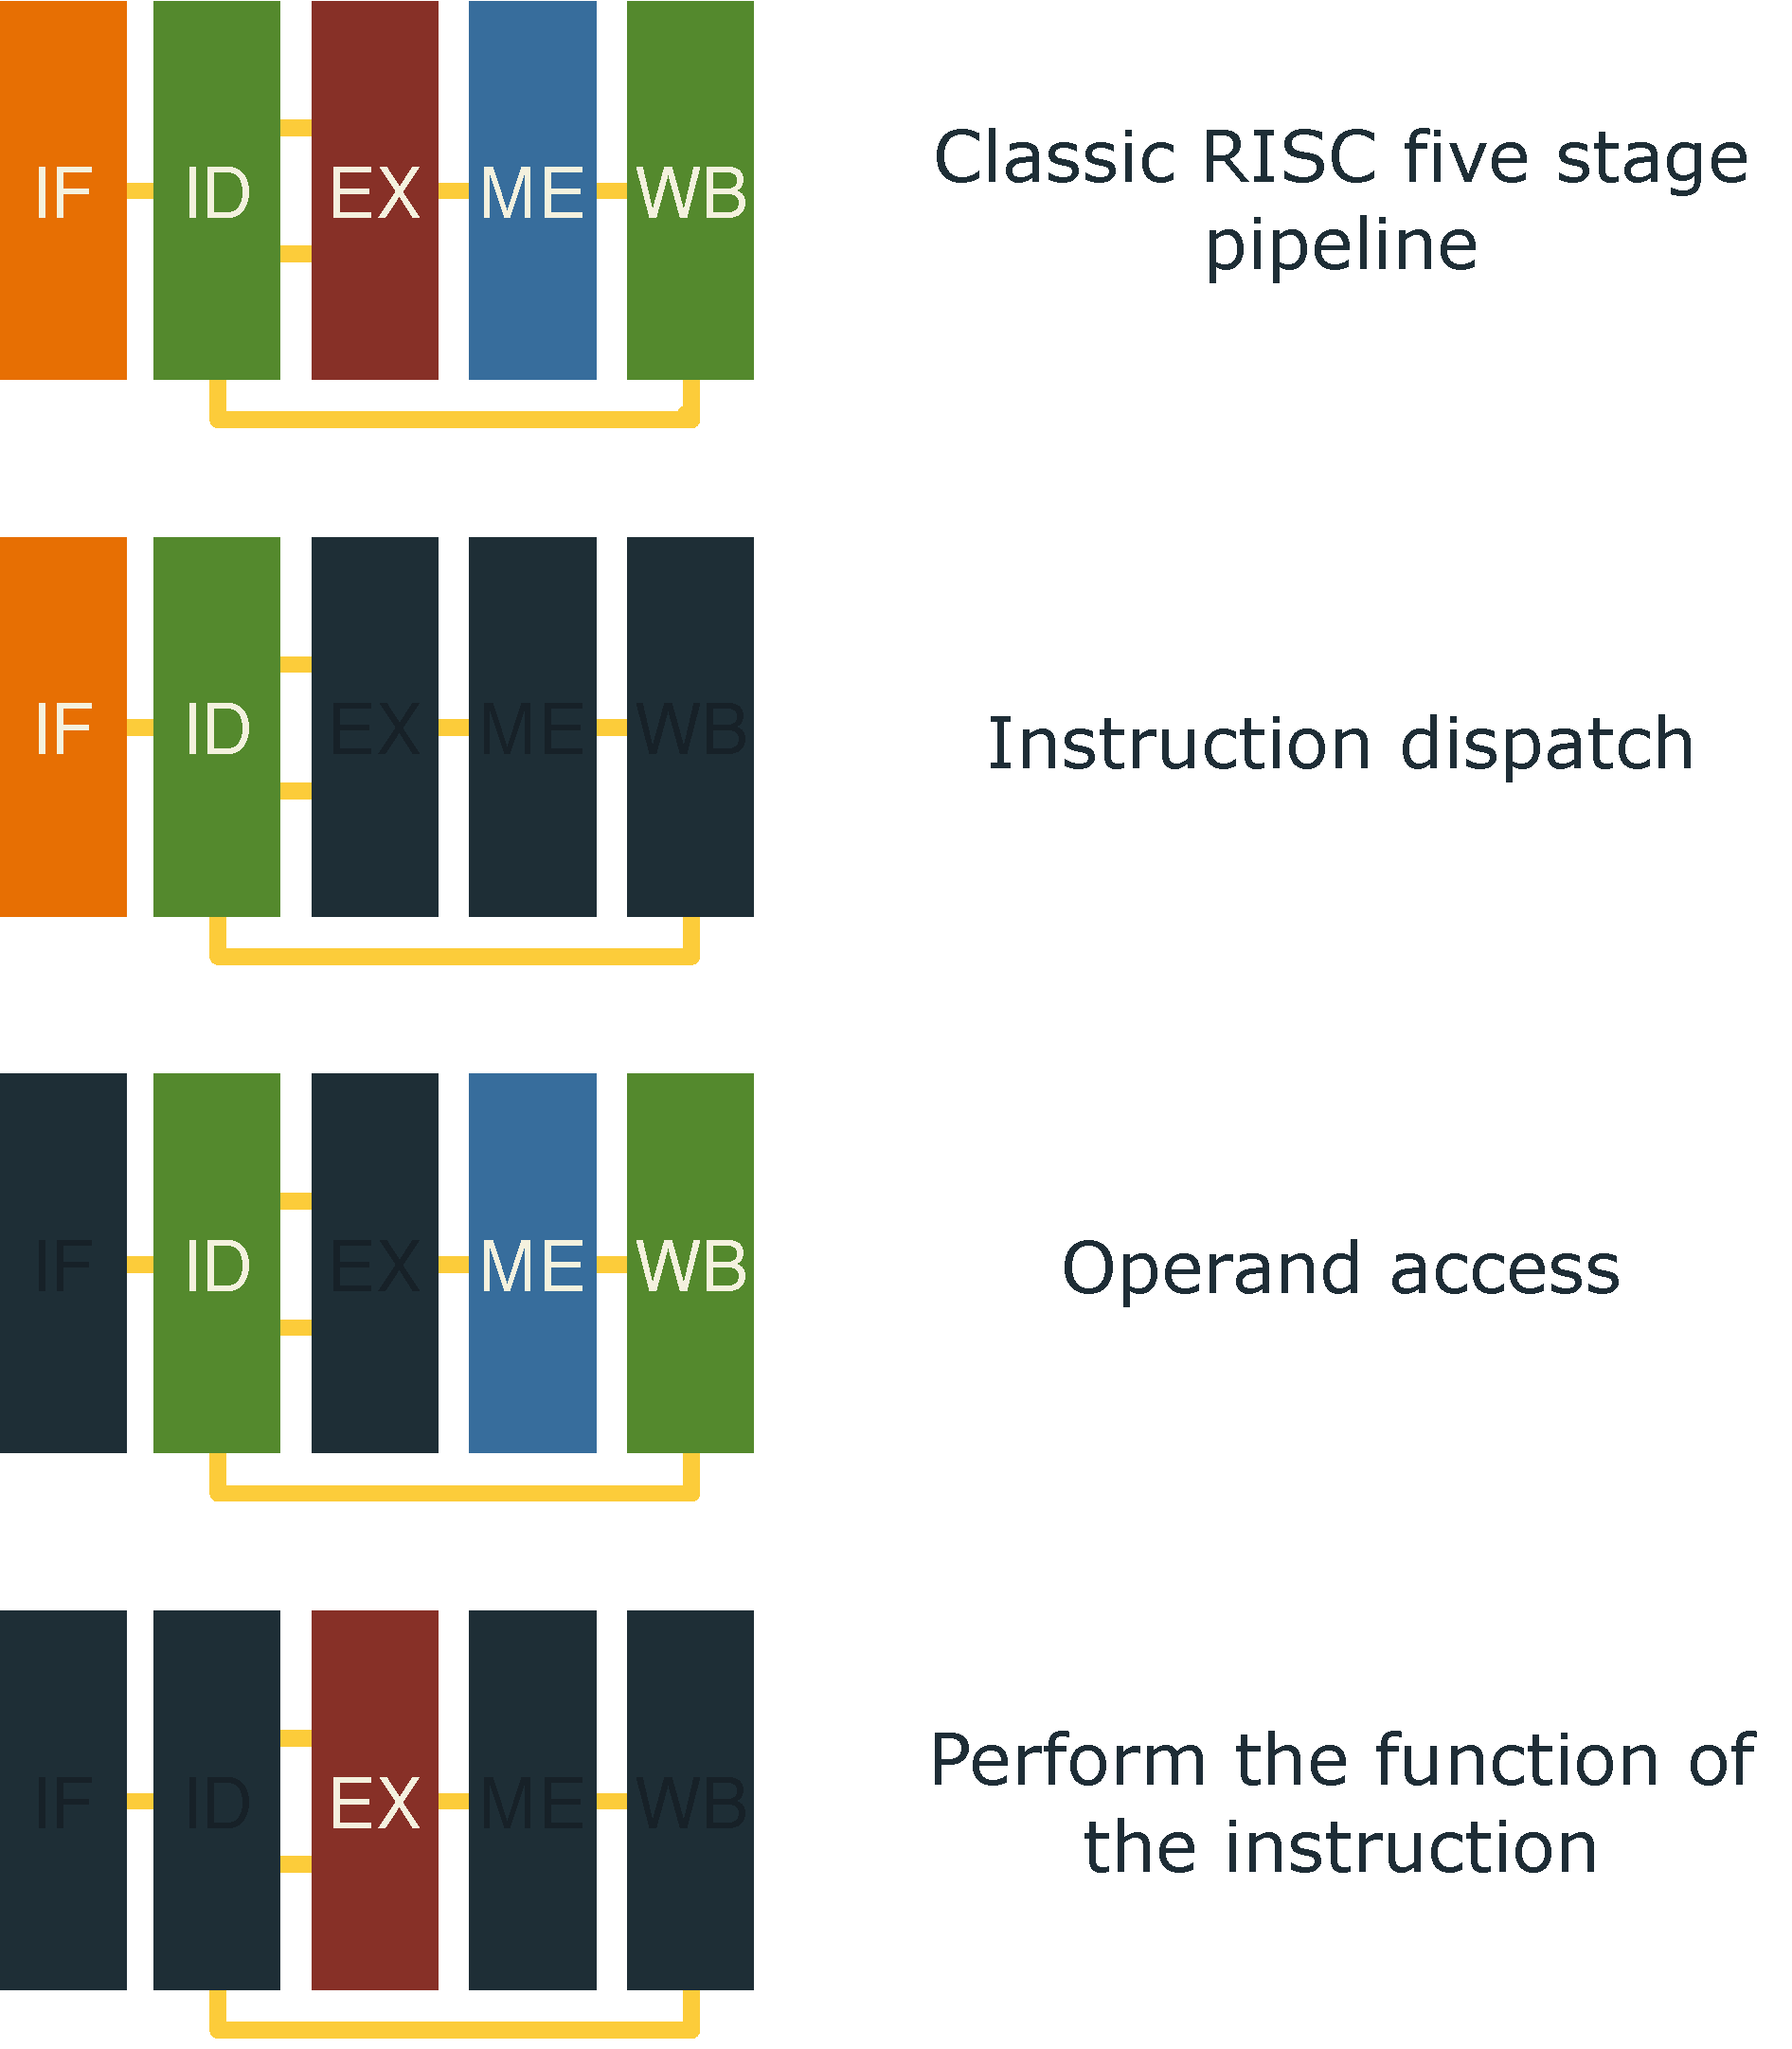
\includegraphics[scale=.25]{figures/ch2-risc-pipeline.pdf}
\caption{Interpretation costs of bytecode interpreters}
\label{fig:interpretation-cost}
\end{figure}

An interesting way to further illustrate the purpose of each interpretation step
from the angle of a virtual machine is to correlate them with the stages in a classic reduced instruction set computer (RISC) pipeline.
Figure~\ref{fig:interpretation-cost} illustrates the five stages in a classic RISC pipeline:
instruction fetch (IF), instruction decode (ID), execute (EX), memory access (ME) and write back (WB).
The instruction dispatch step in bytecode interpreters is similar to instruction fetch and decode stages in RISC.
We can correlate the late stage of instruction decode, memory access and write back in RISC to operand access in an interpreter.
Since these are the stages that prepare the operands for the computing unit and stores the end result back to either a register or memory address.
The interpreter step that performs the function of the instruction works exactly as the execute stage in RISC, which performs the actual computation.

The cost of running a hosted program on an interpreter consists of the costs of performing each of the three steps we described above.
Among those steps, instruction dispatch and operand access does not directly contribute to the actual work of the hosted program.
The less time the interpreter spend in these two steps, the more time the interpreter spend in doing the actual work.
Therefore, an efficient bytecode interpreter must encompass techniques that optimize instruction dispatch and operand access.

\subsection{Switch-based Dispatch}

\begin{figure}[th]
\centering
\subfigure[dispatch loop] {
  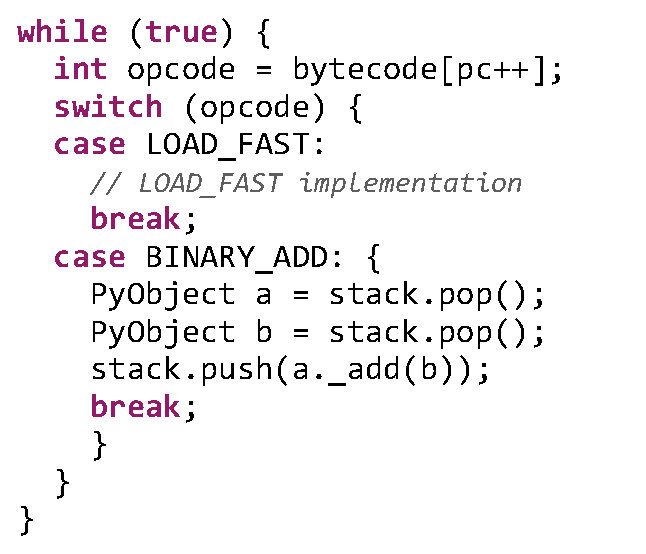
\includegraphics[scale=.70]{figures/ch2-switch-based-dispatch-code.pdf}
  \label{fig:switch-based-dispatch-code}
}
\subfigure[branches in switch-based dispatch] {
  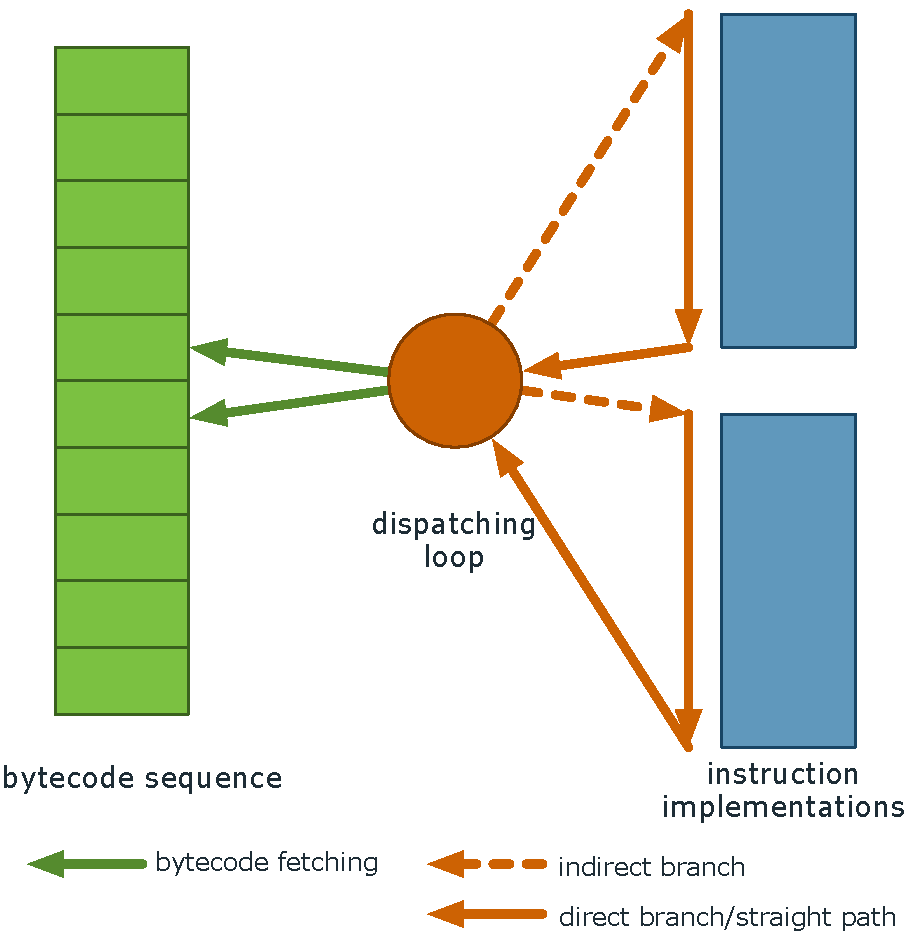
\includegraphics[scale=.47]{figures/ch2-switch-based-dispatch-branch.pdf}
  \label{fig:switch-based-dispatch-branch}
}
\caption{switch-based dispatch}
\label{fig:switch-based-dispatch}
\end{figure}

The simplest way to construct a bytecode interpreter is to use an interpreter loop and a switch statement in the loop to dispatch each bytecode instruction.
Figure~\ref{fig:switch-based-dispatch-code} illustrates a switch-based bytecode interpreter loop written in Java.
In each iteration of the loop, the interpreter fetches the next instruction and use the switch statement to redirect execution to the case block that implements the instruction.
Figure~\ref{fig:switch-based-dispatch-branch} shows the branches involved in a switch-based dispatch.
Note that each iteration of the dispatch loop shares the same indirect branch.
Since the bytecode sequence is input dependent and unlikely to form a predictable pattern,
branch prediction mechanisms in modern hardware tend to mis-predict the shared indirect branch.
This mis-prediction results in a significant performance penalty for switch-based bytecode interpreters.

\section{Efficient Instruction Dispatch Techniques}
\label{sec:efficient-instruction-dispatch-techniques}

\subsection{Direct Threading Dispatch}
\label{sec:direct-threading-dispatch}

\begin{figure}[th]
\centering
\subfigure[direct threading interpreter] {
  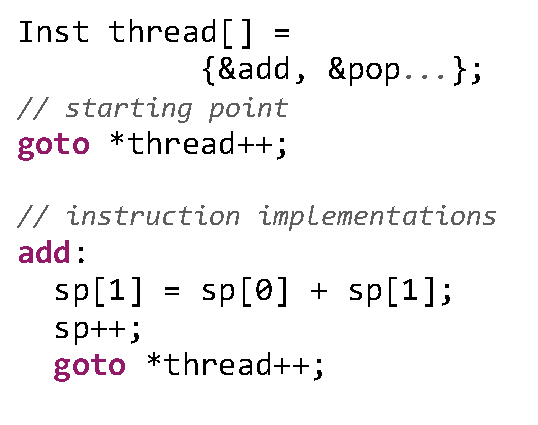
\includegraphics[scale=.85]{figures/ch2-direct-threading-dispatch-code.pdf}
  \label{fig:direct-threading-dispatch-code}
}
\subfigure[branches in direct threading dispatch] {
  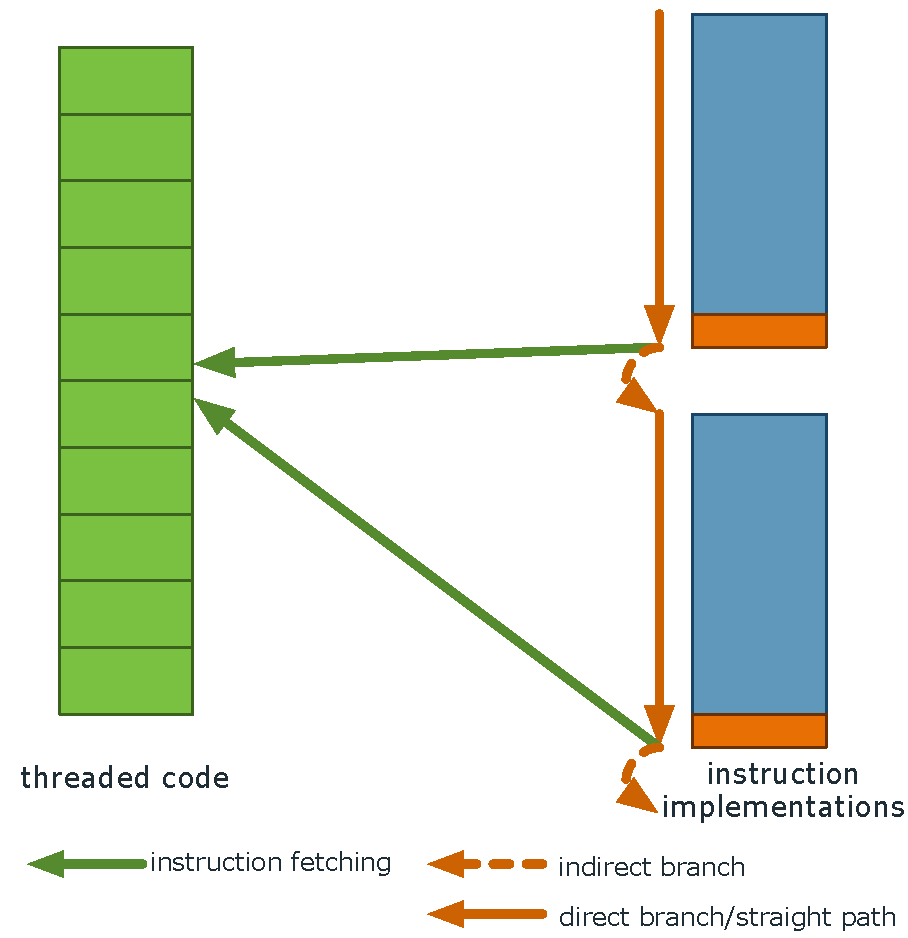
\includegraphics[scale=.47]{figures/ch2-direct-threading-dispatch-branch.pdf}
  \label{fig:direct-threading-dispatch-branch}
}
\caption{direct threading dispatch}
\label{fig:direct-threading-dispatch}
\end{figure}

Instead of letting each instruction dispatch share the same branch, direct threading duplicates instruction dispatch at the end of each instruction implementation~\cite{bell73}.
Figure~\ref{fig:direct-threading-dispatch-code} illustrates this technique written in C.
Direct threading requires an additional translation phase that translates the bytecode sequence into a sequence of pointers or the threaded code.
Each pointer in the threaded code points to the instruction implementation that corresponds to the bytecode instruction in the original bytecode input.
The interpreter starts interpretation by jumping to the address pointed by the first pointer in the threaded code as shown in Figure~\ref{fig:direct-threading-dispatch-code}.
Similarly each instruction implementation repeat the same dispatch routine at the end of it to forward execution to the next instruction implementation.
The duplicated dispatch branches reduce indirect branch mis-predictions.
Therefore, direct threading alleviates the performance loss we have seen in switch-based dispatch.

\subsection{Subroutine Threading Dispatch}

\begin{figure}[th]
\centering
\subfigure[subroutine threaded code] {
  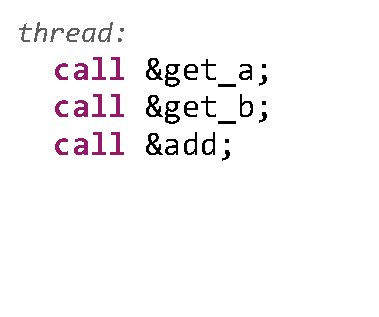
\includegraphics[scale=.85]{figures/ch2-subroutine-threading-dispatch-code.pdf}
  \label{fig:subroutine-threading-dispatch-code}
}
\subfigure[branches in subroutine threading dispatch] {
  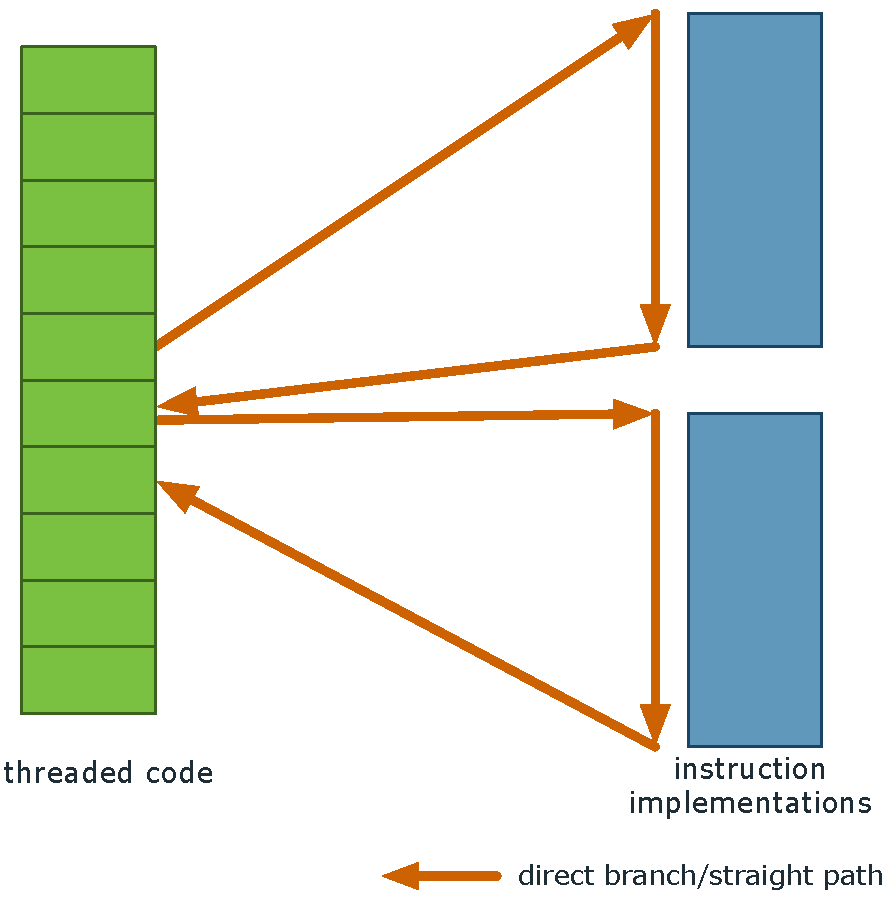
\includegraphics[scale=.47]{figures/ch2-subroutine-threading-dispatch-branch.pdf}
  \label{fig:subroutine-threading-dispatch-branch}
}
\caption{subroutine threading dispatch}
\label{fig:subroutine-threading-dispatch}
\end{figure}

Subroutine threading takes one step further by translating the input bytecode sequence directly to executable machine code.
The translated machine code or the subroutine threaded code is a sequence of machine level calls.
Each call is a direct branch jumping to an instruction implementation as a subroutine.
The subroutine threaded code translation phase translates each input bytecode to a subroutine call to the corresponding instruction implementation.
Each instruction implementation ends with a return instruction that transfer execution back to the threaded code.
Note that the call instruction in subroutine threading is a direct branch.
Although the return instruction is an indirect branch, modern hardware can accurately predict call/return repairs which results in a performance increase.

\section{Efficient Instruction Dispatch for Hosted Bytecode Interpreters}

Instruction dispatch greatly affects the overall performance of a bytecode interpreter.
The implementation of an efficient instruction dispatch technique like the ones explained in Chapter~\ref{sec:efficient-instruction-dispatch-techniques}
relies on the use of computed goto's.
Due to the restricted use of pointers, a hosted bytecode interpreter written in Java can not make use of those techniques.
To address this issue, we extend the JVM by adding the functionality of threaded code generation to enable efficient instruction dispatch for hosted interpreters.
Our research prototype takes an existing switch-based bytecode interpreter written in Java, and converts it into a direct threading interpreter in a semi-automatic fashion.

\subsection{System Overview}

\begin{figure}[th]
\centering
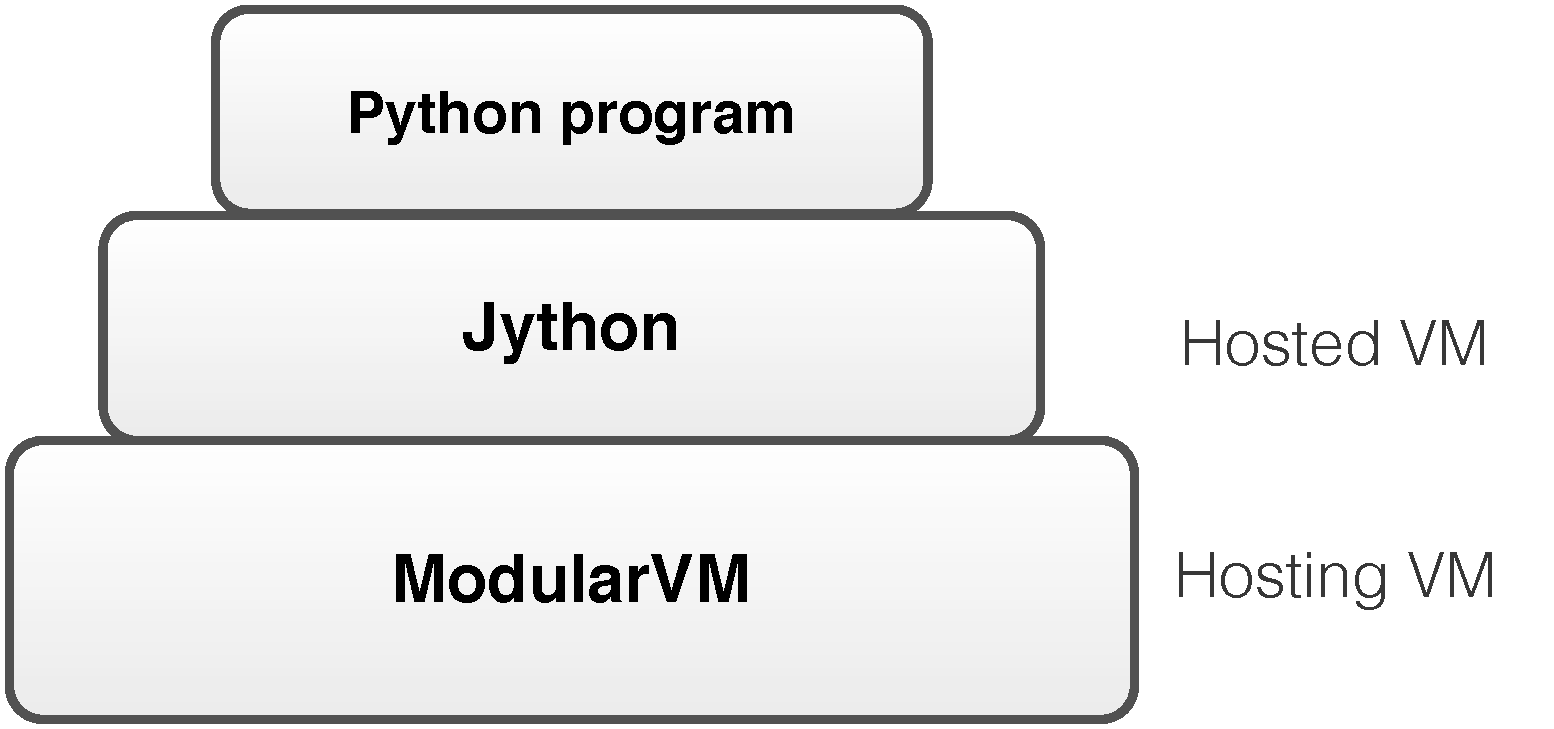
\includegraphics[scale=.3]{figures/ch2-jython-on-modularvm.pdf}
\caption{Jython on ModularVM}
\label{fig:jython-on-modularvm}
\end{figure}

Our system, Modular VM, is an extension to Maxine VM~\cite{Wimmer2013}, a research JVM developed at Oracle Labs.
We build Modular VM with the ability to recognize hosted interpreters running on top of it and automatically optimizes them.
We host Jython, a Python VM written in Java, on Modular VM in our experiment to show case our optimization.
Figure~\ref{fig:jython-on-modularvm} illustrates the overall system setup.
Modular VM hosts Jython like other regular JVMs.
Jython executes Python program in two fashions: using the baseline bytecode interpreter or
compiling Python code to Java bytecode and let the JVM compiler further compile it down to machine code.
Our optimization focuses on the bytecode interpreter.
It shows that by incorporating efficient interpreter optimizations, bytecode interpreter can deliver comparable performance to a basic compiler.

\subsection{Threaded Code Generation}

\begin{figure}[!h]
\centering
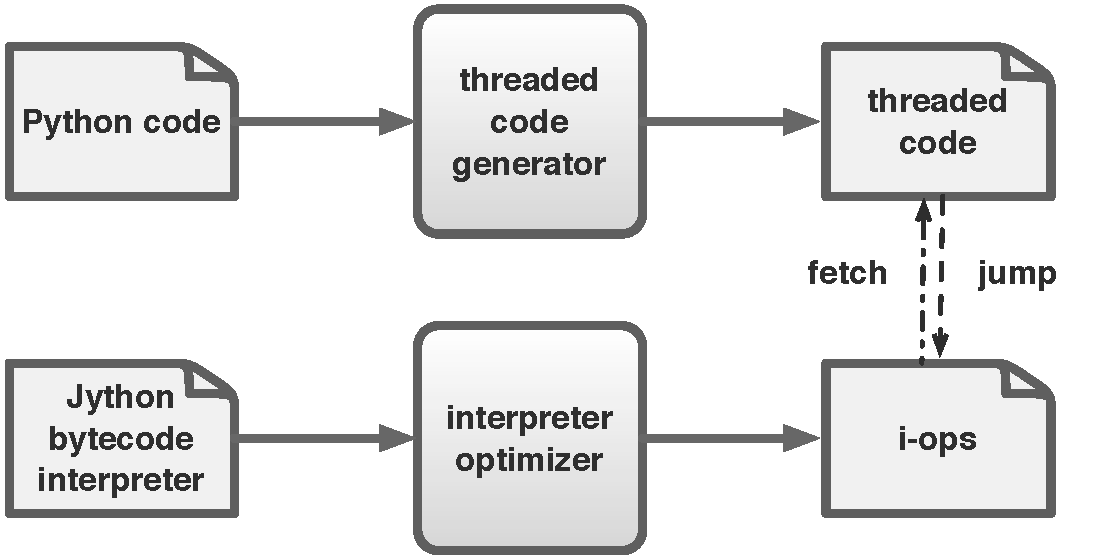
\includegraphics[scale=.5]{figures/ch2-direct-threading-on-modularvm.pdf}
\caption{Threaded code generation}
\label{fig:direct-threading-on-modularvm}
\end{figure}

Modular VM performs threaded code generation in two steps.
First, it recognizes the hosted interpreter running on top of it and transforms it into an optimized one.
To be more specific, Modular VM extracts all the bytecode instruction implementations or i-ops for short from the interpreter and
compiles them into machine code using the existing Java compiler.
Modular VM then initializes an i-op code table that contains the address of all the compiled i-ops.
After this transformation, the interpreter is ready to execute Python programs.
It first translates Python source code to Python bytecode and then further translates bytecode to direct threaded code using the i-op code table.
The generated threaded code is a sequence of code pointers copied from the i-op code table.

Figure~\ref{fig:direct-threading-on-modularvm} illustrates this work flow.
The interpreter optimizer in the Figure applies the transformation to Jython's bytecode interpreter.
Subsequently, the thread code generator produces threaded code and executes it.
Both interpreter optimizer and threaded code generator are part of Modular VM.
Our system encapsulates the details of i-ops compilation and threaded code generation from the hosted VM.

\subsubsection{Interpreter Annotation}

\begin{figure}[ht]
\centering
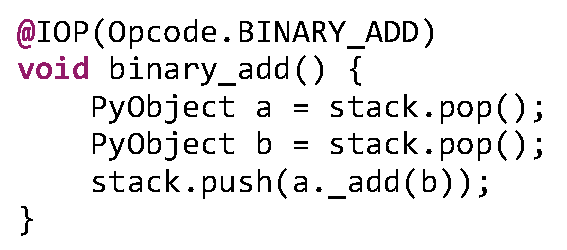
\includegraphics[scale=.65]{figures/ch2-annotated-iop-code.pdf}
\caption{Annotated i-op}
\label{fig:annotated-iop}
\end{figure}

Modular VM uses a Java annotation based domain specific language to integrate with the hosted interpreter.
Our programmable interface provides a set of annotations for hosted VM implementers to annotate different components of their interpreter.
We expect hosted VM implementers to properly annotate the interpreter class, the bytecode class and all the i-op methods for our system to identify the structure of the interpreter.
Figure~\ref{fig:annotated-iop} shows an annotated i-op in Jython's bytecode interpreter refactored to its own separate method.
Modular VM automatically picks up Java methods annotated as i-ops, optimizes them and put them into the i-op code table.

\subsubsection{Next Dispatch}

\begin{figure}[ht]
\centering
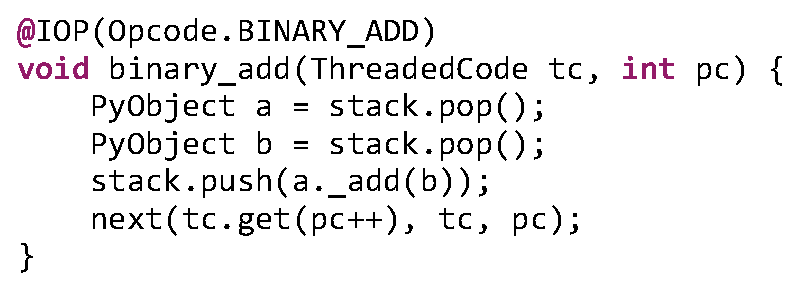
\includegraphics[scale=.65]{figures/ch2-iop-with-next-code.pdf}
\caption{I-op with next dispatch}
\label{fig:iop-with-next}
\end{figure}

Direct threading, as explained in Chapter~\ref{sec:direct-threading-dispatch}, duplicates instruction dispatch at the end of each instruction implementation or i-op.
When the interpreter optimizer compiles an i-op, it also insert a synthesized \emph{next} routine at the end of the i-op.
The \emph{next} routine performs the actual instruction dispatch.
Figure~\ref{fig:iop-with-next} illustrates the i-op of \texttt{BINARY\_ADD} in Jython with the \emph{next} routine.
Note that the figure shows what the program looks like with the added instruction dispatch.
Hosted VM implementers are not required to write the additional code.
As shown in Figure~\ref{fig:iop-with-next}, the intrinsic function \texttt{next} performs an indirect jump to the next i-op in the threaded code.
The \emph{next} routine also passes the reference to the threaded code and virtual program pointer to the next instruction to continue the execution of the program.

\subsubsection{Stack Frame Reusing}

As described above, the \texttt{next} instruction dispatch performs a native indirect branch instead of a call.
Therefore, i-ops need to reuse the same stack frame allocated for each Python function invocation.
We implement this using two special i-ops, \texttt{PROLOGUE} and \texttt{EPILOGUE}.
Both of them are manually assembled instead of compiled from Java source code.
\texttt{PROLOGUE}, used at the beginning of a function, allocates a stack frame that is big enough to accommodate all i-ops.
\texttt{EPILOGUE}, used to model \texttt{RETURN}, deallocates the stack frame and returns.
The interpretation of a Python method always start with a \texttt{PROLOGUE} and end with an \texttt{EPILOGUE}.
Stack frame reusing reduces the number of native machine instructions executed for each hosted virtual machine instruction dispatch.

\subsubsection{Efficient Array Stores}
\label{sec:efficient-array-stores}

Another problem affecting hosted interpreter performance on the JVM is the performance of array stores.
Java being a safe language performs type check such as \texttt{ArrayStoreException} checks on array stores.
Hosted language interpreters like the one in Jython uses an operand stack to manage temporal operands.
Internally, the operand stack is implemented as an Java object array.
During interpretation, every i-op that produces a value performs an array store onto the operand stack.
As a result, the interpreter repeatedly performs the same the type check, even though every i-op is guaranteed to produce an value that is safe to be stored on the operand stack.

We identified the detrimental effect of preserving array type-safety for hosted interpreters.
Our interpreter optimizer omits the \texttt{ArrayStoreException} checks when compiling the i-ops of hosted interpreters.

\subsubsection{An Example}

\begin{figure}[th]
\centering
\subfigure[Python source code] {
  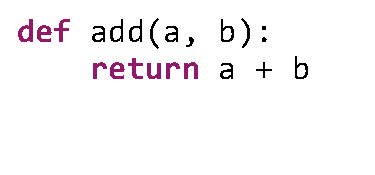
\includegraphics[scale=.85]{figures/ch2-threaded-code-example-python.pdf}
  \label{fig:threaded-code-example-python}
}
\subfigure[Python bytecode] {
  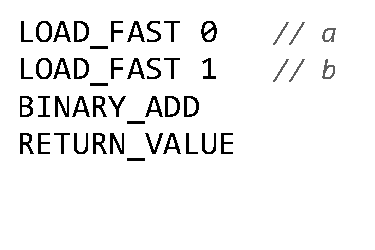
\includegraphics[scale=.75]{figures/ch2-threaded-code-example-bytecode.pdf}
  \label{fig:threaded-code-example-bytecode}
}
\subfigure[Threaded code] {
  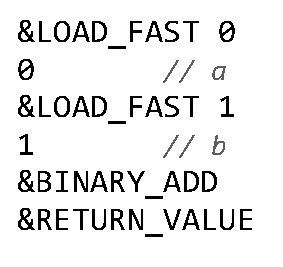
\includegraphics[scale=.7]{figures/ch2-threaded-code-example-threaded-code.pdf}
  \label{fig:threaded-code-example-threaded-code}
}
\caption{Direct threading example}
\label{fig:threaded-code-example}
\end{figure}

Figure~\ref{fig:threaded-code-example} illustrates the Python program translation in Jython hosted on Modular VM.
The input program, as shown in Figure~\ref{fig:threaded-code-example-python}, is a simple Python method that adds two parameters.
Jython first converts the program to the bytecode sequence show in Figure~\ref{fig:threaded-code-example-bytecode}.
Note that the bytecode instruction \texttt{LOAD\_FAST} consists of not only the \texttt{LOAD\_FAST} opcode itself but also an opcode argument ($0$ or $1$) in the bytecode sequence.
Figure~\ref{fig:threaded-code-example-threaded-code} shows the direct threading code produced by the threaded code generator.
Aside from the translated i-op addresses, the threaded code generator also copies opcode arguments, like the one in \texttt{LOAD\_FAST}, into the threaded code.

\section{Evaluation}

\chapter{Hosted AST Interpreter}

Abstract syntax trees, ASTs, are the simplest and most natural ways to implement programming languages.
They do not require an additional translation step that linearizes ASTs produced by the parser to bytecode or other forms of internal representations.
They also lend themselves well to optimizations that are particularly beneficial to highly dynamic languages like Python.

We present ZipPy, a Python 3 implementation that is hosted on the JVM.
ZipPy incorporates recent works on self-optimizing AST interpreters for the JVM.
Our work however focuses on high level guest language features that are distinct in Python and
how well we can fit them onto the existing optimizing AST interpreter framework.

\section{Python on Truffle}

\begin{figure}[t]
\centering
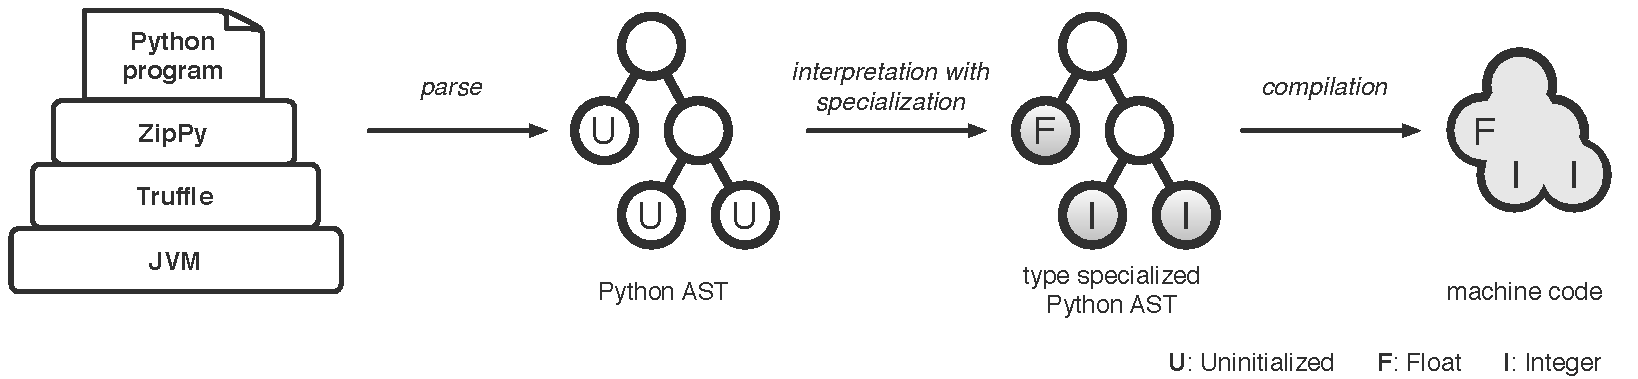
\includegraphics[scale=.6]{figures/ch3-python-on-truffle.pdf}
\caption{Python on Truffle}
\label{fig:python-on-truffle}
\end{figure}

In principle, ``everything'' can change at any moment in dynamic language programs.
This dynamic nature is the major impediment to ahead-of-time optimization.
In practice, however, programmers tend to minimize the rate of change, which makes the code highly predictable.
Types, for instance, typically remain stable between successive executions of a particular operation instance.
Deutsch and Schiffman report that speculative type specialization succeeds $95\%$ of the time in their classic Smalltalk-80 implementation~\cite{Deutsch1984}.

Truffle is a self-optimizing runtime system that makes it easy to perform type specialization for dynamic languages running on top of the JVM~\cite{Wurthinger+13}.
It allows language implementers to implement their guest language by writing an AST interpreter using Java.
An interpreter written in this way enjoys low cost type specialization via automatic node rewriting~\cite{Wurthinger+12,Brunthaler2010inca,Brunthaler2010quickening}.
AST node rewriting collects runtime type information, and speculatively replaces the existing nodes with specialized and more efficient ones.
Subsequently, Truffle just-in-time compiles the specialized AST, written in Java, directly to machine code using the underlying Java compiler.
Upon a type mis-speculation, the specialized AST node handles the type change by replacing itself with a more generic one.
The node replacement triggers deoptimization from the compiled code and transfers execution back to the interpreter.
If the re-specialized AST stays stable, Truffle can again compile it to machine code.

Our system, ZipPy, is a full-fledged prototype Python 3 implementation built atop Truffle.
It leverages Truffle's type specialization feature and its underlying compilation infrastructure (see Figure~\ref{fig:python-on-truffle}).
This architecture helps ZipPy outperform Python implementations that either do not exploit runtime type specialization or lack a just-in-time compiler.
However, Truffle has no knowledge about specific high level guest language semantics, like generators in Python.
Further performance exploration of a guest language will mainly benefit from better insights on distinct features of the language and
making better use of the host compiler based on those insights.
In this thesis we focus on guest language level optimizations we added to ZipPy.

\section{Design and Implementation}

ZipPy benefits from the Truffle framework in two ways.
First, Truffle's Java annotation based domain specific language (DSL) greatly simplifies the implementation of type specialization in dynamic languages like Python~\cite{Humer+2014}.
Second, Truffle bridges the gap between the hosted AST interpreter and the underlying Java JIT compiler.
It empowers the hosted interpreter with the performance of a custom compiler without having the hosted VM implementers to actually write a compiler.
The end performance one could achieve on Truffle usually surpasses that of a custom build class file compiler not to mention the upfront cost of building such compiler.

However, Truffle is not a fool proof framework.
It does require knowledge of the Java compiler internals to make better use of the framework.
In this section we describe the design choices we made to retrofit the core part of the Python language onto Truffle's execution model.

\subsection{Applying Type Specializations}

\begin{figure}[t]
\centering
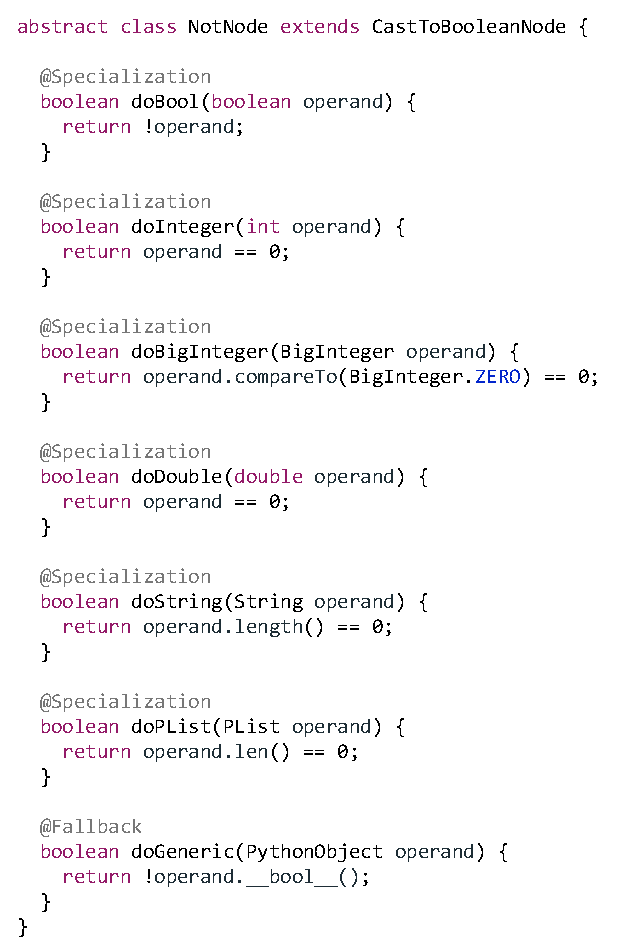
\includegraphics[scale=.8]{figures/ch3-not-node-code.pdf}
\caption{Implementation of \texttt{NotNode} in ZipPy}
\label{fig:not-node-code}
\end{figure}

\begin{figure}[t]
\centering
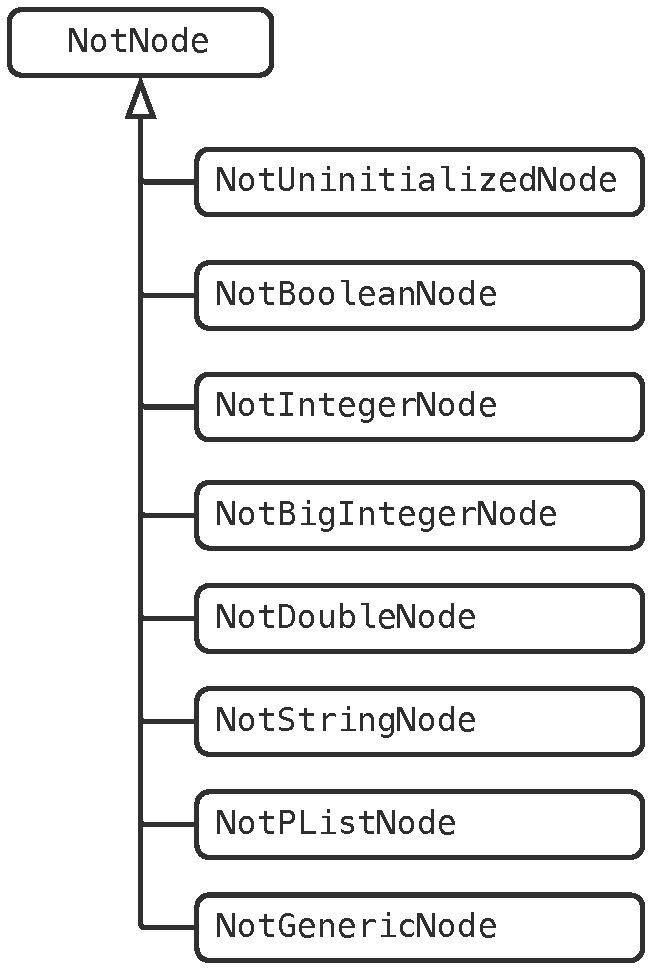
\includegraphics[scale=.5]{figures/ch3-not-node-derivatives.pdf}
\caption{Derivatives of \texttt{NotNode} in ZipPy}
\label{fig:not-node-derivatives}
\end{figure}

Truffle provides a Java annotation based source code generation engine.
Hosted VM implementers can use this engine to automatically generate type specialized derivatives for their AST interpreters.
Derivative generation is an essential but tedious part of applying type specializations.
This code generation process requires little boilerplate code from the hosted VM implementers and helps them to focus on the core logic of their interpreter.

\texttt{not} is a unary arithmetic operation in Python.
The operation evaluates the given expression to a boolean value and returns the inversion of that value.
Similar to other arithmetic operations, ZipPy implements \texttt{not} as a single AST node.
Figure~\ref{fig:not-node-code} illustrates the implementation of the \texttt{NotNode} in ZipPy using Truffle's DSL.
Note that each method annotated using \texttt{@Specialization} represents a type specialized derivative of the \texttt{NotNode}.
For instance, the method \texttt{doInteger} and \texttt{doDouble} implement the \texttt{not} operation for integers and floating point numbers.
We will explain in~\ref{sec:numeric-types} about the reason why we specialize against Java primitive types instead of boxed representations of numeric types in Python.
\texttt{@Fallback} denotes the generic version of the \texttt{not} operand.

Truffle's code generation engine produces the actual implementation of the derivative nodes.
Figure~\ref{fig:not-node-derivatives} shows the derivative classes produced by Truffle.
It generates a class for each method annotated with \texttt{@Specialization} in Figure~\ref{fig:not-node-code}.
The derivative nodes perform node rewriting based type specialization at runtime.
As shown in Figure~\ref{fig:python-on-truffle}, a \texttt{NotNode} starts with the uninitialized version.
At runtime, the node rewrites itself to a derivative that matches the type of the incoming operand.
The rewrite follows the order of the classes shown in Figure~\ref{fig:not-node-derivatives} from the top to the bottom.
If no matching derivative is found, the node rewrites to \texttt{NodeGenericNode}, which perform the generic routine for the \texttt{not} operation.

\subsection{Numeric Types}
\label{sec:numeric-types}

\subsection{Comnposite Data Types}

\chapter{Generator Peeling}
\label{chp:ch4-peeling}

Generators offer an elegant way to express iterators.
However, performance has always been their Achilles heel and has prevented widespread adoption.
We present techniques to efficiently implement and optimize generators.

We have implemented our optimizations in ZipPy, a modern, light-weight AST interpreter based Python 3 implementation targeting the Java virtual machine.
Our implementation builds on a framework that optimizes AST interpreters using just-in-time compilation.
In such a system, it is crucial that AST optimizations do not prevent subsequent optimizations.
Our system was carefully designed to avoid this problem.
We report an average speedup of \peelingSpeedup{}$\times$ for generator-bound programs.
As a result, using generators no longer has downsides and programmers are free to enjoy their upsides.

\section{Motivation}

Many programming languages support generators, which allow a natural expression of iterators.
We surveyed the use of generators in real Python programs, and found that among the 50 most popular Python projects
listed on the Python Package Index (PyPI)~\cite{pypi} and GitHub~\cite{github}, 90\% of these programs use generators.

Generators provide programmers with special control-flow transfers that allows function executions to be suspended and resumed.
Even though these control-flow transfers require extra computation, the biggest performance bottleneck is caused by preserving the state of a function between a suspend and a resume.
This bottleneck is due to the use of \emph{cactus} stacks required for state preservation.
Popular language implementations, such as CPython~\cite{python}, and CRuby~\cite{ruby}, allocate frames on the heap.
Heap allocation eliminates the need for cactus stacks, but is expensive on its own.
Furthermore, function calls in those languages are known to be expensive as well.

In this thesis, we examine the challenges of improving generator performance for Python.
First, we show how to efficiently implement generators in abstract syntax tree (AST) interpreters,
which requires a fundamentally different design than existing implementations for bytecode interpreters.
We use our own full-fledged prototype implementation of Python 3, called ZipPy\footnote{Publicly available at \url{https://bitbucket.org/ssllab/zippy}},
which targets the Java virtual machine (JVM).
ZipPy uses the Truffle framework~\cite{Wurthinger+13} to optimize interpreted programs in stages, first collecting type feedback in the AST interpreter,
then just-in-time compiling an AST down to optimized machine code.
In particular, our implementation takes care not to prevent those subsequent optimizations.
Our efficient generator implementation optimizes control-transfers via suspend and resume.

Second, we describe an optimization for frequently used idiomatic patterns of generator usage in Python.
Using this optimization allows our system to allocate generator frames to the native machine stack, eliminating the need for heap allocation.
When combined, these two optimizations address both bottlenecks of using generators in popular programming languages, and finally give way to high performance generators.

\noindent{}Summing up, our contributions are:

\begin{itemize}
\item We present an efficient implementation of generators for AST based interpreters that is easy to implement and enables efficient optimization offered by just-in-time compilation.
\item We introduce \emph{generator peeling}, a new optimization that eliminates overheads incurred by generators.
\end{itemize}

\section{Generators in Python}

A generator is a more restricted variation of a coroutine~\cite{grune1977view,Moura2009}.
It encompasses two control abstractions: \emph{suspend} and \emph{resume}.
\emph{Suspend} is a generator exclusive operation, while only the caller of a generator can \emph{resume} it.
Suspending a generator always returns control to its immediate caller.
Unlike regular subroutine calls, which start executing at the beginning of the callee, calls to a \emph{suspended} generator resume
from the point where it most recently suspended itself.
Those two operations are asymmetric as opposed to the symmetric control \emph{transfer} in coroutines.

\subsubsection*{Generator Functions}

\begin{figure}
\centering
\subfigure[Simple generator]{
	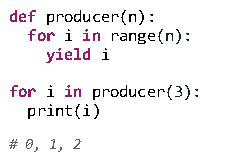
\includegraphics[scale=1.5]{figures/ch4-simple-generator-example-code}
	\label{fig:ch4-simple-generator-code}
}
\subfigure[Python iterator protocol]{
	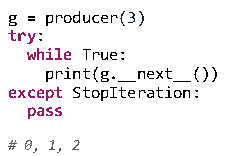
\includegraphics[scale=1.5]{figures/ch4-loop-on-generator-code}
	\label{fig:ch4-iterate-on-generator-code}
}
\caption{A simple generator function in Python}
\label{fig:ch4-generator-example}
\end{figure}

In Python, using the \texttt{yield} keyword in a function definition makes the function a generator function.
A call to a generator function returns a generator object without evaluating the body of the function.
The returned generator holds an execution state initialized using the arguments passed to the call.
Generators implement Python's iterator protocol, which includes a \texttt{\_\_next\_\_} method.
The \texttt{\_\_next\_\_} method starts or resumes the execution of a generator.
It is usually called implicitly, e.g., by a for loop that iterates on the generator (see Figure~\ref{fig:ch4-simple-generator-code}).
When the execution reaches a \texttt{return} statement or the end of the generator function, the generator raises a \texttt{StopIteration} exception.
The exception terminates generator execution and breaks out of the loop that iterates on the generator.
Figure~\ref{fig:ch4-iterate-on-generator-code} shows the desugared version of the for loop that iterates over the generator object \texttt{g} by explicitly calling \texttt{\_\_next\_\_}.

\subsubsection*{Generator Expressions}

\begin{figure}[h]
\centering
\subfigure[Generator expression]{
	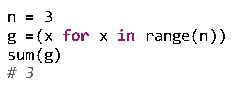
\includegraphics[scale=1.5]{figures/ch4-genexp-example-code}
	\label{fig:ch4-simple-genexp-code}
}
\subfigure[Desugared generator function]{
	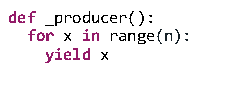
\includegraphics[scale=1.5]{figures/ch4-genexp-desugared-code}
	\label{fig:ch4-genexp-desugared-code}
}
\caption{A simple generator expression in Python}
\label{fig:ch4-genexp-example}
\end{figure}

Generator expressions offer compact definitions of simple generators in Python.
Generator expressions are as memory efficient as generator functions, since they both create generators that lazily produce one element at a time.
Programmers use these expressions in their immediate enclosing scopes.
Figure~\ref{fig:ch4-genexp-example} shows a simple generator expression and its equivalent, desugared generator function definition.
A generator expression defines an anonymous generator function, and directly returns a generator that uses the anonymous function definition.
The returned generator encapsulates its enclosing scope, if the generator expression references symbols in the enclosing scope (\texttt{n} in Figure~\ref{fig:ch4-genexp-example}).
The function \texttt{sum} subsequently consumes the generator by iterating on it in a loop and accumulating the values produced by the generator.

\subsubsection*{Idiomatic Uses of Generators}

\begin{figure}[h]
\centering
\subfigure[Generator loop]{
	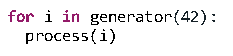
\includegraphics[scale=1.5]{figures/ch4-idiomatic-generator-loop-code}
	\label{fig:ch4-idiomatic-loop-code}
}
\subfigure[Implicit generator loop]{
	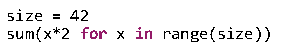
\includegraphics[scale=1.5]{figures/ch4-idiomatic-implicit-loop-code}
	\label{fig:ch4-idiomatic-implicit-code}
}
\caption{Idiomatic uses of generators}
\label{fig:ch4-idiomatic-patterns}
\end{figure}

The idiomatic way of using generators in Python is to write a \emph{generator loop}.
As shown in Figure~\ref{fig:ch4-idiomatic-loop-code}, a generator loop is a for loop that calls a generator function and consumes the returned generator object.
The common use pattern of a generator expression is to use it as a closure and pass it to a function that consumes it (see Figure~\ref{fig:ch4-idiomatic-implicit-code}).
The consumer functions, like \texttt{sum}, usually contain a loop that iterates on the generator.
Therefore, we refer to this pattern as an \emph{implicit generator loop}.
Explicit and implicit generator loops cover most of the generator usage in Python programs.
Our generator peeling optimization, which we explain in Section~\ref{sec:ch4-generaor-peeling}, targets these patterns.

\section{Generators Using an AST Interpreter}

Java, the host language of Truffle and ZipPy, does not offer native support for coroutines.
Our AST interpreter needs to model the semantics of generators.
However, the conventional way of implementing generators in a bytecode interpreter does not work in an AST setting.
In this section, we discuss the challenges of supporting generators in an AST interpreter, and present the solution we devised for ZipPy.

\subsection{AST Interpreters vs. Bytecode Interpreters}

\begin{figure}
\centering
\subfigure[Implementation of \texttt{WhileNode}]{
	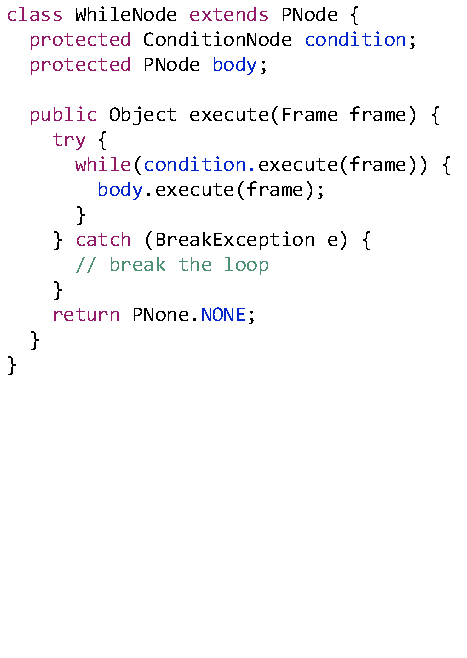
\includegraphics[scale=.9]{figures/ch4-while-node-code}
	\label{fig:ch4-while-node-code}
}
\subfigure[Implementation of \texttt{GenWhileNode}]{
	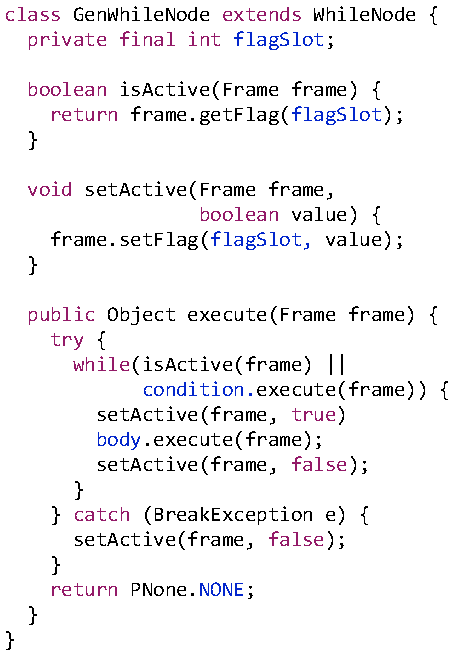
\includegraphics[scale=.9]{figures/ch4-gen-while-node-code}
	\label{fig:ch4-gen-while-node-code}
}
\caption{Two different \texttt{WhileNode} versions}
\label{fig:ch4-while-nodes}
\end{figure}

The de-facto Python implementation, CPython, uses bytecode interpretation.
It parses the Python program into a linearized bytecode representation and executes the program using a bytecode interpreter.
A bytecode interpreter is \emph{iterative}.
It contains an interpreter loop that fetches the next instruction in every iteration and performs its operation.
The bytecode index pointing to the next instruction is the only interpreter state that captures the current location of the program.
The interpreter only needs to store the program activation and the \emph{last} bytecode index when the generator suspends.
When resuming, a generator can simply load the program activation and the \emph{last} bytecode index before it continues with the next instruction.

An AST interpreter on the other hand is \emph{recursive}.
The program evaluation starts from the root node, then recursively descends to the leaves, and eventually returns to the root node.
In ZipPy, every AST node implements an \texttt{execute} method (see Figure~\ref{fig:ch4-while-nodes}).
Each \texttt{execute} method recursively calls the \texttt{execute} methods on its child nodes.
The recursive invocation builds a native call stack that captures the current location of the program.
The interpreter has to save the entire call stack when the generator suspends.
To resume the generator execution, it must rebuild the entire call stack to the exact point where it last suspended.

\subsection{Generator ASTs}
\label{sec:ch4-generator-ast}

ZipPy stores local variables in a heap-allocated frame object.
AST nodes access variables by reading from and writing to dedicated frame slots.
During just-in-time compilation, Truffle is able to map frame accesses to the machine stack and eliminate frame allocations.
However, a generator needs to store its execution state between a suspend and resume.
The frame object must therefore be kept on the heap which prevents Truffle's frame optimization.

In general, our AST interpreter implements control structures using Java's control structures.
We handle non-local returns, i.e., control flow from a deeply nested node to an outer node in the AST, using Java exceptions.
Figure~\ref{fig:ch4-genfunc-before} illustrates the AST of a Python generator function.
We model loops or if statements using dedicated \emph{control nodes}, e.g., a \texttt{WhileNode}.
The \texttt{BlockNode} groups a sequence of nodes that represents a basic block.
The \texttt{YieldNode} performs a non-local return by throwing a \texttt{YieldException}.
The exception bypasses the two parent \texttt{BlockNode}s, before the \texttt{FunctionRootNode} catches it.
The \texttt{FunctionRootNode} then returns execution to the caller.

\subsubsection*{Generator Control Nodes}

\begin{figure}
\centering
\subfigure[Before translation]{
	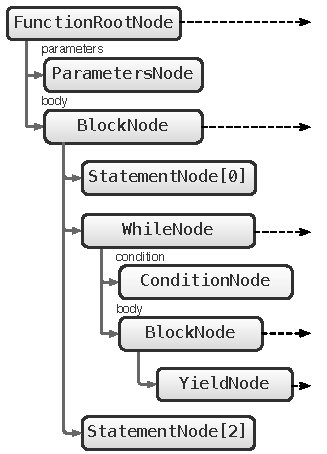
\includegraphics[scale=1.1]{figures/ch4-gen-function-orig}
	\label{fig:ch4-genfunc-before}
}
\subfigure[Translated]{
	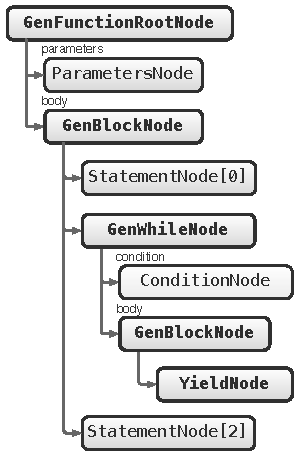
\includegraphics[scale=1.1]{figures/ch4-gen-function-translated}
	\label{fig:ch4-genfunc-translated}
}
\caption{Translation to generator AST}
\label{fig:ch4-genfunc-translation}
\end{figure}

Every control node in ZipPy has a local state stored in the local variables of its \texttt{execute} method.
The local state captures the current execution of the program, for instance, the current iterator of a for loop node or the current node index of a block node.
To support generators we decide to implement an alternative generator version for each control node.
These control nodes do not rely on local state, and keep all execution state in the frame.
However, it is overly conservative to use generator control nodes everywhere in a generator function.
We only need to use generator control nodes for the parent nodes of \texttt{YieldNode}s, since a yield operation only suspends the execution of these nodes.

Figure~\ref{fig:ch4-while-node-code} shows the implementation of a \texttt{WhileNode}.
Note that the loop condition result is a local state of the node stored in the call stack of its \texttt{execute} method.
When a \texttt{YieldException} is thrown somewhere in the loop body, it unwinds the call stack and discards the current loop condition result.
When the generator resumes, it will not be able to retrieve the previous loop condition result without re-evaluating the \texttt{condition} node.
The re-evaluation may have side effects and violate correct program behavior.
Therefore, this implementation only works for normal functions but not for generator functions.

Figure~\ref{fig:ch4-gen-while-node-code} shows the generator version of the \texttt{WhileNode}, the \texttt{GenWhileNode}.
It keeps an \emph{active} flag, a local helper variable, in the frame.
The \texttt{execute} method accesses the flag by calling the \texttt{isActive} or \texttt{setActive} method.
When a yield occurs in the loop body, the active flag remains true.
When resuming, it bypasses the condition evaluation and forwards execution directly to the loop body.

Note that it is incorrect to store the active flag as a field in the \texttt{GenWhileNode}.
Different invocations of the same generator function interpret the same AST, but should not share any state stored in the AST.
An alternative way to implement a \texttt{GenWhileNode} is to catch \texttt{YieldException}s in the \texttt{execute} method and set the active flag in the catch clause.
This implementation requires the \texttt{GenWhileNode} to re-throw the \texttt{YieldException} after catching it.
If we implement generator control nodes in this way, a yield operation will cause a chain of Java exception handling which is more expensive than the solution we chose.

Similar to the \texttt{GenWhileNode}, we implement a generator version for all the other control nodes in ZipPy.
Every generator control node has its own active flags stored in the frame.
The descriptions of the generator control nodes are as follows:

\begin{itemize}

\item \texttt{GenFunctionRootNode}:
Stores an active flag in the frame.
Only applies arguments when the flag is false.
Resets the flag and throws \texttt{StopIteration} exception upon termination of the generator.

\item \texttt{GenBlockNode}:
Stores the current node index in the frame.
Skips the executed nodes when the index is not zero.
Resets the index to zero upon exit.

\item \texttt{GenForNode}:
Stores the current iterator in the frame.
Resets the iterator to \texttt{null} upon exit.

\item \texttt{GenIfNode}:
Similar to \texttt{GenWhileNode}, uses an active flags to indicate which branch is active.

\item \texttt{GenWhileNode}:
See Figure~\ref{fig:ch4-gen-while-node-code}.

\item \texttt{GenBreakNode}:
Resets active flags of the parent control nodes up to the targeting loop node (the innermost enclosing loop), including the loop node.

\item \texttt{GenContinueNode}:
Resets active flags of the parent control nodes up to the targeting loop node, excluding the loop node.

\item \texttt{YieldNode}:
Must be a child of a \texttt{GenBlockNode}.
Evaluates and stores the yielding value in the frame before throwing the \texttt{YieldException}.
The root node then picks up the value and returns it to the caller.
The \texttt{YieldNode} also advances the statement index of its parent \texttt{BlockNode} to ensure that the generator resumes from the next statement.

\end{itemize}

\subsubsection*{Control Node Translation}
\label{sec:ch4-ast-of-gen-func}

ZipPy first parses Python functions into ASTs that use the \emph{normal} control nodes.
Generator functions require an additional translation phase that replaces the \emph{normal} control nodes with their \emph{generator} equivalents.
Figure~\ref{fig:ch4-genfunc-translation} illustrates this translation.
We only replace the control nodes that are parents of the \texttt{YieldNode}s, since these nodes fully capture the state required to suspend and resume execution.

The translated generator AST always keeps a snapshot of its execution in the frame.
When resuming, it is able to retrieve all the necessary information from the snapshot and rebuild the entire interpreter call stack to the exact point where it left off.

The flag accesses in the generator control nodes and the exception based control flow handling add performance overheads.
However, the underlying compiler is able to compile the entire generator AST into machine code.
It also optimizes control flow exceptions and converts them to direct jumps.
The jumps originate from where the exception is thrown and end at the location that catches it.
The AST approach, enforced by the underlying framework, does add complexity to the implementation of generators.
However, the performance gains offset this slight increase of the implementation effort.

\subsubsection*{Yield as an Expression}

\begin{figure}[h]
\centering
\subfigure[Yield expression]{
	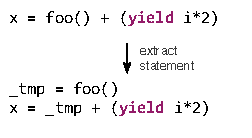
\includegraphics[scale=1.45]{figures/ch4-yield-expression-example}
	\label{fig:ch4-yield-expression-example}
}
\subfigure[Translated multiply]{
	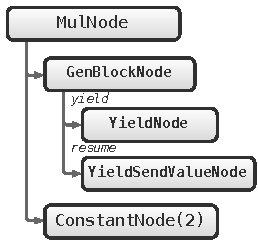
\includegraphics[scale=1.1]{figures/ch4-yield-expression-ast}
	\label{fig:ch4-yield-expression-ast}
}
\caption{Translation of a yield expression}
\label{fig:ch4-yield-expression}
\end{figure}

Python allows programmers to use yield in expressions.
A yield expression returns a value passed from the caller by calling the generator method \texttt{send}.
This enhancement allows the caller to pass a value back to the generator when it resumes, and brings generators closer to coroutines.
However, it requires generator ASTs to be able to resume to a specific expression.

Figure~\ref{fig:ch4-yield-expression-example} shows an example of yield expressions.
The assignment statement to variable \texttt{x} consumes the value returned by the yield expression.
Figure~\ref{fig:ch4-yield-expression-ast} shows the translated AST of the multiplication sub-expression.
Note that we translate the yield expression to a \texttt{GenBlockNode} containing a \texttt{YieldNode} and a \texttt{YieldSendValueNode}.
When the \texttt{YieldNode} suspends execution, it advances the active node index of the parent \texttt{GenBlockNode} to point to the next node.
This action ensures that the generator restarts execution from the \texttt{YieldSendValueNode}, which returns the value sent from the caller.

In a more complicated case, the statement consuming the yield expression could contain sub-expressions with a higher evaluation order.
In other words, the interpreter should evaluate these expressions before the yield expression.
Some of them could have side effects, i.e., the call to \texttt{foo} in Figure~\ref{fig:ch4-yield-expression-example}.
To avoid re-evaluation, we convert such expressions into separate statements and create variables to store the evaluated values.
When the generator resumes, it picks up the evaluated values from the variables without visiting the expression nodes again.

\section{Optimizing Generators with Peeling}
\label{sec:ch4-generaor-peeling}

Generator peeling is an AST level speculative optimization that targets the idiomatic generator loop pattern.
It transforms the high level generator calling semantics to lower level control structures and eliminates the overheads incurred by generators altogether.

\subsection{Peeling Generator Loops}

\begin{figure}[ht]
\centering
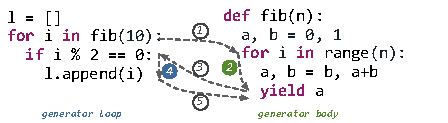
\includegraphics[scale=1.5]{figures/ch4-gen-exec-order}
\caption{Program execution order of a generator loop}
\label{fig:ch4-gen-exec-order}
\end{figure}

Figure~\ref{fig:ch4-gen-exec-order} shows a generator loop (left) that collects even numbers among the first ten Fibonacci numbers generated by \texttt{fib} (right) into the list \texttt{l}.
For each iteration in the loop, the program performs the following steps:

\begin{enumerate}
\item Call \texttt{\_\_next\_\_} on the generator and resume execution.

\item Perform another iteration in the for \texttt{range} loop to compute the next Fibonacci number.

\item Return the value of \texttt{a} to the caller and assign it to \texttt{i}.

\item Execute the body of the generator loop.

\item Return to the loop header and continue with the next iteration.
\end{enumerate}

Among those steps listed above, only step two and four perform the actual computation.
Steps one and three are generator specific resume and suspend steps.
They involve calling a function, resuming the generator AST to the previous state and returning the next value back to the caller.
Those generator specific steps add high overhead to the real work in the generator loop.

The most common and effective technique for optimizing function calls is to inline callees into callers.
However, traditional function inlining does not work for generators.
The desugared generator loop (similar to the one shown in Figure~\ref{fig:ch4-iterate-on-generator-code}) includes two calls: one to the generator function \texttt{fib} and another one to the \texttt{\_\_next\_\_} method.
The call to \texttt{fib} simply returns a generator object during loop setup, and is not performance critical.
Inlining the call to \texttt{\_\_next\_\_} requires special handling of \emph{yield}s rather than treating them as simple returns.
An ideal solution should handle both calls at the same time, while still preserving semantics.

Observe that the generator loop always calls \texttt{\_\_next\_\_} on the generator unless it terminates.
If the generator loop body was empty, we can replace the loop with the generator body of \texttt{fib} and still preserve semantics.
Furthermore, assuming the above mentioned replacement is in-place, for the non-empty loop body case, we can replace each yield statement with the generator loop body.
Figure~\ref{fig:ch4-peeling-trans} illustrates this transformation.
The solid arrow depicts the generator loop replacement that ``inlines'' the generator body.
The dashed arrow shows the yield replacement that combines the generator code and the caller code.

Figure~\ref{fig:ch4-fib-peeled} shows the pseudo-code of the transformed program.
We combine the generator body and the loop body in the same context.
The original call to the generator function \texttt{fib} translates to the assignment to \texttt{n} which sets up the initial state of the following generator body.
The generator body replaces the original generator loop.
We simplify the yield statement to a single assignment.
The assignment transfers the value of \texttt{a} from the generator body to the following loop body.
The loop body in turn consumes the ``yielded'' value of \texttt{i}.

\begin{figure}[!t]
\centering
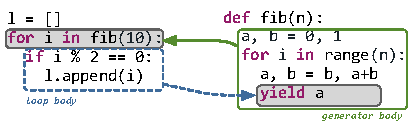
\includegraphics[scale=1.5]{figures/ch4-peeling-generator-call}
\caption{Peeling transformation}
\label{fig:ch4-peeling-trans}
\end{figure}

\begin{figure}[!t]
\centering
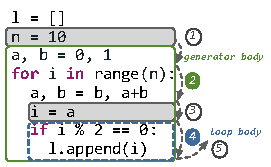
\includegraphics[scale=1.5]{figures/ch4-fib-peeled}
\caption{Transformed generator loop}
\label{fig:ch4-fib-peeled}
\end{figure}

The transformation peels off the generator loop, and removes both calls, to \texttt{fib} and \texttt{\_\_next\_\_}.
The optimized program does not create a generator object.
It eliminates the step one and simplifies the step three shown in Figure~\ref{fig:ch4-gen-exec-order}.
These two steps do not contribute to the real computation.
The numbers on the right of Figure~\ref{fig:ch4-fib-peeled} denote the corresponding execution steps of the original generator loop shown in Figure~\ref{fig:ch4-gen-exec-order}.
The two assignments preceding the transformed generator body and the loop body (grayed in Figure~\ref{fig:ch4-fib-peeled}) preserve the correct data flow into and out of the generator code.

We simplified the pseudo code shown in Figure~\ref{fig:ch4-fib-peeled} for clarity.
Our transformation is not limited to the case where the call to the generator function happens at the beginning of the consuming loop.
If the creation of the generator object happens before the loop, we apply the same transformation that combines the generator body with the loop body.
We explain the actual AST transformation in more detail in Section~\ref{sec:ch4-ast-transformation}.

\subsection{Peeling AST Transformations}
\label{sec:ch4-ast-transformation}

\begin{figure*}
\centering
\subfigure[AST transformation]{
	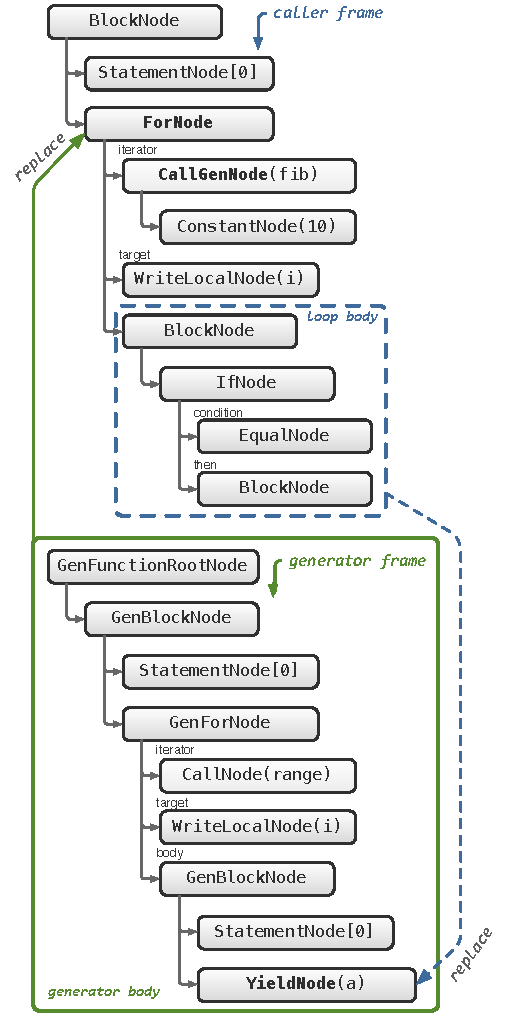
\includegraphics[scale=.82]{figures/ch4-ast-before-peeling}
	\label{fig:ch4-ast-before-peeling}
}
\subfigure[Transformed generator loop AST]{
	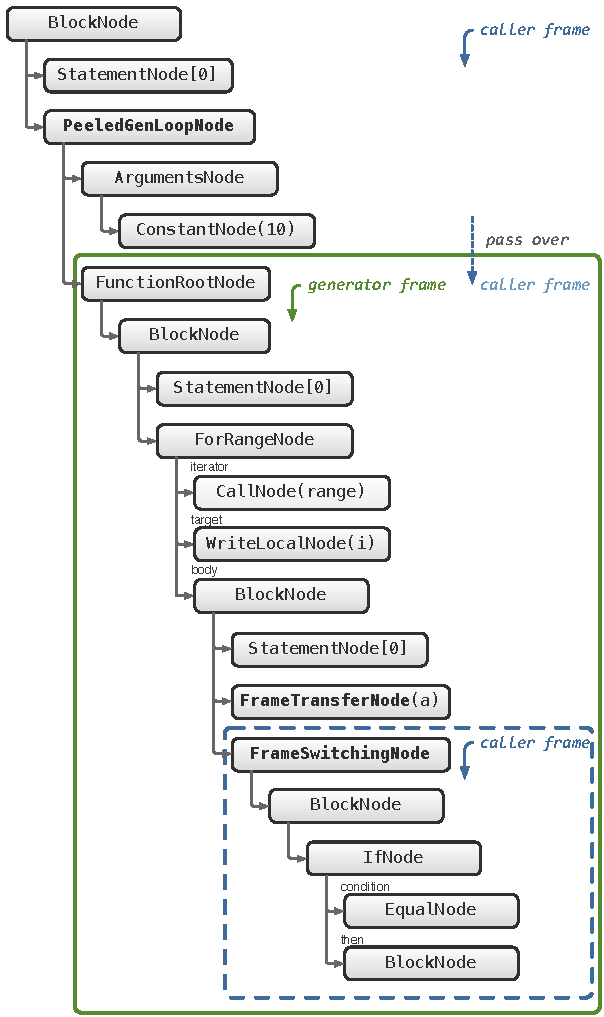
\includegraphics[scale=.82]{figures/ch4-peeled-ast}
	\label{fig:ch4-peeled-ast}
}
\caption{Peeling AST transformation}
\label{fig:ch4-ast-transformation}
\end{figure*}

Figure~\ref{fig:ch4-ast-before-peeling} shows the AST transformation of our Fibonacci example.
The upper half of the figure shows the AST of the generator loop.
The AST contains a \texttt{CallGenNode} that calls the generator function \texttt{fib}, and returns a generator object to its parent node.
The parent \texttt{ForNode} representing the for loop then iterates over the generator.
The lower half of the figure shows the AST of the generator function \texttt{fib}.
Note that the generator body AST uses generator control nodes and includes the \texttt{YieldNode} that returns the next Fibonacci number to the caller.

The figure also illustrates the two-step peeling AST transformation.
First we replace the \texttt{ForNode} that iterates over the generator with the AST of the generator body.
Second, we clone the AST of the loop body and use it to replace the \texttt{YieldNode} in the generator body.
Figure~\ref{fig:ch4-peeled-ast} shows the result of the transformation.
We use a \texttt{PeeledGenLoopNode} to guard the transformed generator body.
The \texttt{PeeledGenLoopNode} receives the arguments from the \texttt{ArgumentsNode} and passes them the transformed generator body.
The \texttt{FrameTransferNode} transfers the Fibonacci number stored in the variable \texttt{a} to the following loop body (equivalent to step three in Figure~\ref{fig:ch4-fib-peeled}).
The transformed loop body in turn consumes the ``yielded'' number.

ZipPy implements a number of different versions of \texttt{PeeledGenLoopNode} to handle different loop setups.
For instance, a generator loop could consume an incoming generator object without calling the generator function at the beginning of the loop.
The transformed \texttt{PeeledGenLoopNode} in this case guards against the actual call target wrapped by the incoming generator object and receives the arguments from the generator object.

\subsection{Polymorphism and Deoptimization}
\label{sec:ch4-polymorphic-and-deopt}

ZipPy handles polymorphic operations by forming a chain of specialized nodes with each node implementing a more efficient version of the operation for a particular operand type.
The interpreter then dispatches execution to the desired node depending on the actual type of the operand.
Like other operations in Python, the type of the iterator coming into a loop can change at runtime.
A loop that iterates over multiple types of iterators is a polymorphic loop.

\begin{figure}
\centering
\subfigure[Monomorphic]{
	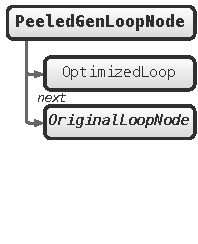
\includegraphics[scale=1.15]{figures/ch4-ast-peeled-mono}
	\label{fig:ch4-ast-peeled-mono}
}
\subfigure[Polymorphic]{
	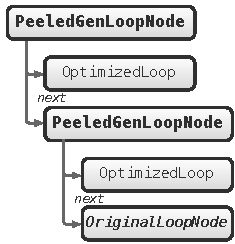
\includegraphics[scale=1.15]{figures/ch4-ast-peeled-poly}
	\label{fig:ch4-ast-peeled-poly}
}
\subfigure[Deoptimized]{
	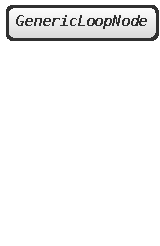
\includegraphics[scale=1.15]{figures/ch4-ast-peeled-deopt}
	\label{fig:ch4-ast-peeled-deopt}
}
\caption{Handling of polymorphic generator loop}
\label{fig:ch4-peeling-polymorphic}
\end{figure}

Generator peeling is a loop specialization technique that targets generators, a particular kind of iterators.
ZipPy handles polymorphic loops by forming a chain of specialized loop nodes including \texttt{PeeledGenLoopNode}s.
A \texttt{PeeledGenLoopNode} checks the actual call target of the incoming iterator before it executes the optimized loop.
As shown in Figure~\ref{fig:ch4-peeling-polymorphic}, if the target changes, then the execution falls through to the original loop node.
ZipPy is able to apply an additional level of the generator peeling transformation for the new iterator type if it happens to be a generator as well.

However, forming a polymorphic chain that is too deep could lead to code explosion.
If the depth of the chain goes beyond a pre-defined threshold, ZipPy stops optimizing the loop and replaces the entire chain with a generic loop node.
The generic loop node is capable of handling all types of incoming iterators but with limited performance benefit.

\subsection{Frames and Control Flow Handling}
\label{sec:ch4-frame-and-control}

The AST of the optimized generator loop combines nodes from two different functions and therefore accesses two different frame objects.
Programmers can use non-local control flows such as \texttt{break}s or \texttt{continue}s in a generator loop body.
We explain how to handle frames and such control flows in the rest of this section.

\subsubsection*{Frame Switching}

% two frames in the fig
The transformed AST illustrated in Figure~\ref{fig:ch4-peeled-ast} accesses two frames: the caller frame and the generator frame.
Figure~\ref{fig:ch4-two-frames} shows the layouts of the two frames.
The nodes belonging to the caller function read from and write to the caller frame to access its local variables.
The generator body nodes do so through the generator frame.
The \texttt{PeeledGenLoopNode} allocates the generator frame and passes it to the dominated generator body.
To enable caller frame access in the deeply nested loop body, the node also passes over the caller frame.
Therefore, in the sub-tree dominated by the \texttt{PeeledGenLoopNode}, both frames are accessible.

\begin{figure}[!ht]
\centering
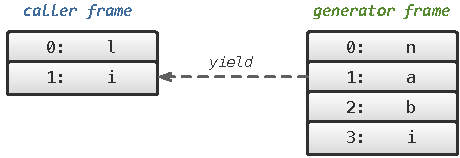
\includegraphics[scale=1.2]{figures/ch4-two-frames}
\caption{The caller and generator frame objects of the Fibonacci example}
\label{fig:ch4-two-frames}
\end{figure}

% passing caller over and switches between two frames
Although keeping both frames alive and accessible, the interpreter picks one frame object as the current frame and retains the other one as the background frame.
It passes the current frame to every \texttt{execute} method of the AST nodes as an argument for faster access.
The current frame stores a reference to the background frame.
The accesses to the background frame require one more level of indirection.

In the generator body shown in Figure~\ref{fig:ch4-peeled-ast}, the interpreter sets the generator frame as the current frame.
The \texttt{FrameTransferNode} propagates the values of \texttt{a} in the generator frame to \texttt{i} in the caller frame.
This value propagation corresponds to step 3 in Figure~\ref{fig:ch4-gen-exec-order} and Figure~\ref{fig:ch4-fib-peeled}.
The following \texttt{FrameSwitchingNode} swaps the positions of the two frames and passes the caller frame as the current frame to the dominated loop body.

% truffle remove frame allocation.
Truffle's underlying JIT compiler optimizes frame accesses.
It eliminates frame allocations as long as references to the frame object are not stored on the heap.
A generator stores its execution state by keeping a frame object reference on the heap.
Therefore, the generator AST introduced in Section~\ref{sec:ch4-generator-ast} prevents this frame optimization.
After generator peeling, however, the program does not create and iterate over generators.
It is not necessary to adopt generator control nodes in the ``inlined'' generator body and store frame object references on the heap.
As a result, the compiler can successfully optimize frame accesses in the transformed generator loop regardless of the number of frames.

For generator functions containing multiple yields, we apply the same transformation to each \texttt{YieldNode}.
The resulting AST contains more than one loop body, hence multiple \texttt{FrameSwitchingNode}s.
We rely on the control-flow optimizations of the underlying compiler to minimize the cost of this replication.

Merging both frames could also guarantee correct frame accesses in the transformed AST.
However, this approach is more complicated.
Merging frames combines the allocations of both frames, which requires redirecting all frame accesses to the combined frame.
Upon deoptimization, we need to undo the merge and redirect all frame accesses back to their separate frames.
This process become more complex for the nested generator loop scenario which we explain more in Section~\ref{sec:ch4-multilevel-peeling}.
Since the underlying compiler is able to optimize multiple frame objects, merging frames does not produce faster code.

\subsubsection*{Breaks and Continues}

\begin{figure}
\centering
\subfigure[Break handling]{
	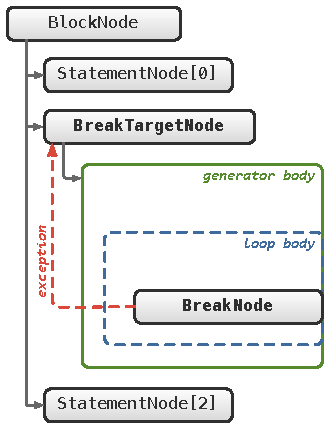
\includegraphics[scale=1.1]{figures/ch4-break-handling}
	\label{fig:ch4-break-handling}
}
\subfigure[Continue handling]{
	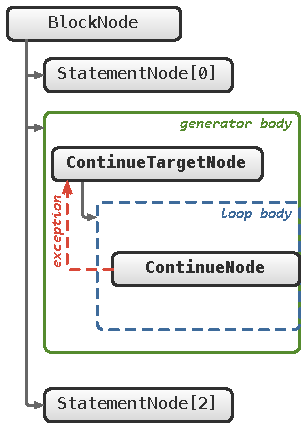
\includegraphics[scale=1.1]{figures/ch4-continue-handling}
	\label{fig:ch4-continue-handling}
}
\caption{Complex control flow handling}
\label{fig:ch4-break-and-continue}
\end{figure}

ZipPy implements break and continue statements using Java exceptions.
A \texttt{BreakNode} throws a break exception, and then a parent node catches the exception.
The control flow exception skips all the nodes between the throwing node and the catching node.
The location of the catch clause determines what the exception can skip.
Figure~\ref{fig:ch4-gen-while-node-code} shows the catch clause in a \texttt{GenWhileNode}.
The node catches the break exception after the while loop, hence the exception breaks the loop.
Similarly, a continue exception caught in the loop body quits the current iteration and continues with the next iteration.
There are no labeled break or continue statements in Python.
Thus, a control flow exception does not go beyond its enclosing loop.
Furthermore, we can extract the exception catch clauses to dedicated nodes to construct more complicated control structures.

A generator loop body may contain break or continue statements that target the generator loop.
Generator peeling replaces the generator loop and embeds the loop body inside the generator body.
To properly handle breaks in the loop body, we interpose a \texttt{BreakTargetNode} between the caller and the generator body as shown in Figure~\ref{fig:ch4-break-handling}.
The nested \texttt{BreakNode} throws a dedicated break exception to skip the generator body, before it reaches the \texttt{BreakTargetNode}.
After catching the exception, the \texttt{BreakTargetNode} returns to its parent and skips the rest of the generator loop.
We handle continues by interposing a \texttt{ContinueTargetNode} between the loop body and the generator body (see Figure~\ref{fig:ch4-continue-handling}).
A continue exception skips the rest of the nodes in the loop body and returns execution to the generator body.
This control flow is equivalent to what a continue does in the original generator loop, that is resuming the generator execution from the statement after the last yield.

The above mentioned interposition is only necessary when the optimized loop body contains break or continue statements.
As we explained in Section~\ref{sec:ch4-ast-of-gen-func}, the underlying compiler optimizes control-flow exceptions into direct jumps.
Therefore, the exception-based control handling has no negative impact on peak performance.

\subsection{Implicit Generator Loops}

\begin{figure}[th]
\centering
\subfigure[Original]{
	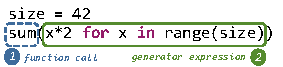
\includegraphics[scale=1.5]{figures/ch4-implicit-orig}
	\label{fig:ch4-implicit-orig}
}

\subfigure[Inlined]{
	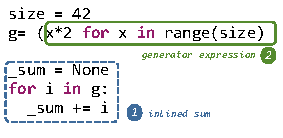
\includegraphics[scale=1.5]{figures/ch4-implicit-inlined}
	\label{fig:ch4-implicit-inlined}
}

\subfigure[Desugared]{
	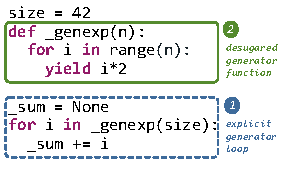
\includegraphics[scale=1.5]{figures/ch4-implicit-desugared}
	\label{fig:ch4-implicit-desugared}
}
\caption{Implicit generator loop transformation}
\label{fig:ch4-implicit-gen-loop}
\end{figure}

An implicit generator loop consists of a generator expression that produces a generator, and a function call that consumes the generator.
ZipPy applies additional transformation on implicit generator loops to enable further optimizations such as generator peeling.

Figure~\ref{fig:ch4-implicit-gen-loop} illustrates this two-step process.
First, we inline the function \texttt{sum} to expose the loop that consumes the generator (see Figure~\ref{fig:ch4-implicit-inlined}).
The inlining step triggers an escape analysis of all the generator expressions in the current scope.
If our analysis finds a generator expression such that the generator it produces does not escape the current scope and
a generator loop that consumes the produced generator exists, ZipPy desugars the expression to a generator function (see Figure~\ref{fig:ch4-implicit-desugared}).
Note that the desugared generator function redirects the references to the enclosing scope to the argument accesses in the local scope.
This redirection eliminates non-local variables in the generator expression and allows the compiler optimization for the enclosing frame.
The desugaring also replaces the generator reference in the inlined loop to a function call.
The transformation exposes the explicit generator loop that we can optimize using generator peeling.

One obstacle when optimizing an implicit generator loop is that the function consuming the generator can be a Python built-in function.
Programmers can use any built-in function that accepts iterable arguments in an implicit generator loop.
Table~\ref{tab:ch4-builtins} lists all the Python 3 built-in functions that accept iterables and divides them into three different categories:

\begin{table}[!ht]
  \begin{center}
    \begin{tabular}{ c c c }
      \toprule
      1. Implement in                & 2. Synthesize to loop & 3. No loop \\
      Python                         &                       & \\
      \midrule
      \texttt{all}, \texttt{any}     & \texttt{bytes}        & \texttt{iter} \\
      \texttt{bytearray}             & \texttt{dict}         & \texttt{next} \\
      \texttt{enumerate}             & \texttt{frozenset}    &               \\
      \texttt{filter}, \texttt{list} & \texttt{set}          &               \\
      \texttt{map}, \texttt{max}     & \texttt{tuple}        &               \\
      \texttt{min}, \texttt{sorted}  &                       &               \\
      \texttt{sum}, \texttt{zip}     &                       &               \\
      \bottomrule
    \end{tabular}
    % \nocaptionrule{}
    \caption{Python Built-in functions that accept iterables}
    \label{tab:ch4-builtins}
  \end{center}
\end{table}

\begin{enumerate}

\item \textbf{Implement in Python}:
Convenience functions that one can write in pure Python.
ZipPy implements these functions using Python code.
They share the same inlining approach with user defined functions.

\item \textbf{Synthesize to loop}:
Constructors of immutable data types in Python.
Cannot be written in pure Python without exposing internal data representations of the language runtime.
The current solution is to speculatively intrinsify the built-in call by replacing the call node with a synthesized AST.
The synthesized AST contains the generator loop and constructs the desired data type.
The intrinsified call site exposes the generator loop and enjoys the same peeling optimization.

\item \textbf{No loop}:
Contains no loop.
We exclude them from the optimization.

\end{enumerate}

\subsection{Multi-level Generator Peeling}
\label{sec:ch4-multilevel-peeling}

ZipPy relies on the tiered execution model of the underlying framework.
It starts executing a Python program in interpretation mode.
The interpreter collects runtime information and inlines function calls that are hot.
We apply function inlining using an inlining budget.
This budget helps to prevent code explosions caused by inlining too many calls or too big a callee.
We perform generator peeling when a generator function call becomes hot, and possibly bail out if the transformation did not succeed.
Generator peeling shares its budget with function inlining.
If a generator peeling transformation is going to overrun the inlining budget, ZipPy aborts the transformation.
After exhausting all possible inlining and peeling opportunities, Truffle compiles the entire AST into machine code.
All subsequent calls to the compiled function execute at peak performance.

\begin{figure}
\centering
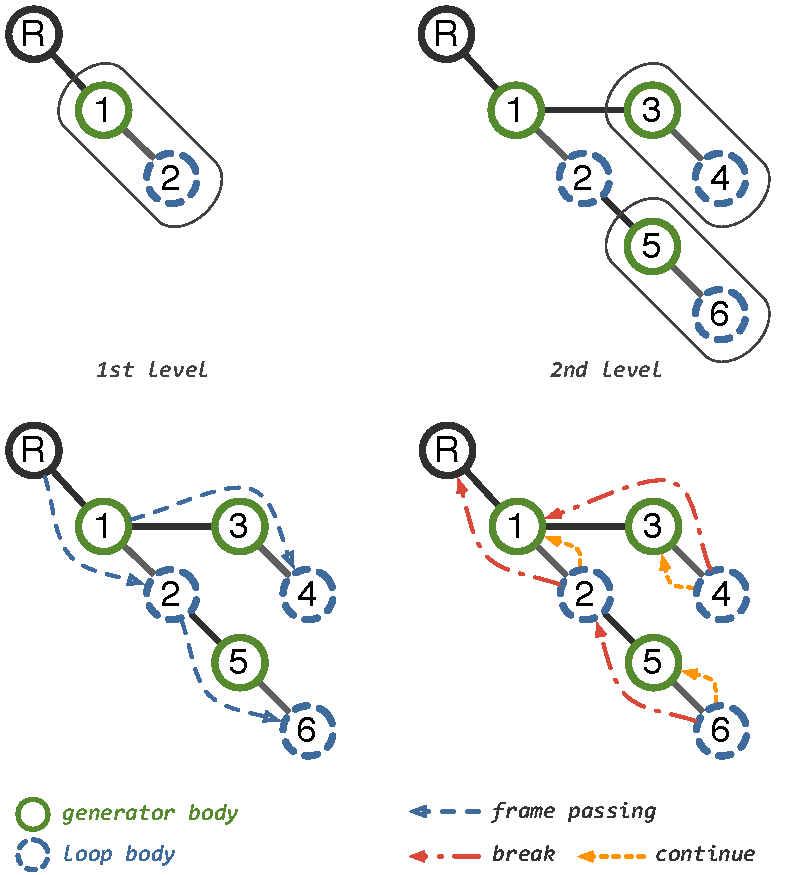
\includegraphics[scale=.9]{figures/ch4-multilevel-peeling}
\caption{Multi-level generator peeling}
\label{fig:ch4-multilevel-peeling}
\end{figure}

An optimized generator loop might include another generator loop.
We call these cases nested generator loops.
Python programs can contain arbitrary levels of nested generator loops.
Our optimization is capable of handling multiple levels of nested generator loops by iteratively peeling one loop layer at a time.
It requires minimal modifications to our existing algorithms to handle this scenario.

Figure~\ref{fig:ch4-multilevel-peeling} shows the AST of three nested generator loops after peeling transformations.
In a simple case, an optimized generator loop consists of two parts: the inlined generator body and the embedded loop body.
To illustrate the relationships between these two program regions, we simplify the structure of the AST by using one node for each program region.
A numbered solid circle denotes a generator body, and a numbered dashed circle denotes a loop body.
An ``inlined'' generator body node is always associated with a loop body node as its immediate child.
As shown in Figure~\ref{fig:ch4-multilevel-peeling}, the first level peeling results in node one being the generator body and node two being the loop body.
The second level peeling includes two optimized generator loops with nodes three and four extended from the generator body and nodes five and six extended from the loop body.
Note that at any level in the tree, a next level peeling can either extend from the generator body or the loop body of the current level.
More complicated cases recursively repeat the same tree structure as shown in Figure~\ref{fig:ch4-multilevel-peeling}.
Therefore, a working solution for the shown tree structure automatically extends to more complicated cases.

% rules in the tree
The tree shown in the figure adheres to the following rules:
Since it is a tree, every node only has one parent except the root node.
Every solid node has an associated dashed node as its child but possibly not the only child.
Every dashed node has an associated solid node as its only parent.
Every dashed node must have one and only one grandparent.

The arrows in Figure~\ref{fig:ch4-multilevel-peeling} depict the desired frame and control-flow handling.
Every dashed node receives two frames: one from its parent and another one from its grandparent.
Since every dashed node has a unique parent and a unique grandparent, there it no ambiguity on which two frames it receives.
A \texttt{continue} returns from a dashed node to its associated solid node.
Since the associated solid node is its only parent, no node can intercept this control-flow.
Our existing algorithms therefore automatically cover frame handling and continue statements for nested generator loops.

Break statements are more complicated.
A \texttt{break} returns from a dashed node to its grandparent.
However, its solid parent node may be the break target of another node and intercept the break exception.
For instance, node one in the figure might catch the break exception thrown in node two or node four.
This ambiguity may cause an incorrect break from node two.
To resolve this issue, we need to label the overlapping break exceptions to filter out undesired ones.
Since it is rare to have two nested generator loops that both use breaks, we consider this scenario as a corner case.

In summary, our peeling transformation is able to handle arbitrary levels of nested generator loops.

\chapter{Optimizing Object Model and Calls}
\label{chp:ch5-object}

Python is an object oriented programing language.
It is a common practice for programmers to encapsulate state and logic using classes in Python programs.
As an implementation of the Python language, it is essential for us to ensure the performance of object operations and method calls in ZipPy.
In the previous chapters we discussed how we optimize arithmetics (Chapter~\ref{chp:ch3-zippy}) and accelerate iterators (Chapter~\ref{chp:ch4-peeling}).
In this chapter we explain how we implement object operations and calls in ZipPy.

\section{Object Model}
\label{sec:ch5-object-module}

\subsection{Python Object Data Representations}

In Python all data is an object.
CPython, the original implementation of Python, constructs every data type in Python as a heap allocated data structure.
Since it is written in C, CPython implements Python built-in data types using C struct and user defined types using hash maps.
This model results in expensive arithmetic operations due to frequent accesses and allocations of data structures in the heap.
Hash map based object model is also inefficient.
Although the cost of hash map operations is amortized for large data sets, the overhead of retrieving or updating a single map entry is still expensive.
In a hash map based object model, retrieving the value of an object field, or an object attribute in Python, is equivalent to reading the value of a map entry.
This operation involves a hashing calculation and a few steps of memory accesses before reaching the memory address that stores the target value.
On the other hand, in a traditional programming language like Java, an object field access, if optimized, is simply a single memory read.
In summary, object model inefficiency is the main impediment to the performance of popular dynamic languages like Python.

\subsubsection{Jython's Object Model Design}

Existing JVM based Python implementations like Jython, however, replicate the same object model design we saw in CPython.
The main approach they took is porting the existing design from C to Java hoping that the underlying Java compiler will magically optimize it.
This approach failed to realize that, although, the java JIT compiler is powerful, its strength is in compiling and optimizing programs written in Java,
the first class citizen of the JVM.
Hence, without additional knowledge to the guest language, the Java compiler is unable to address the miss match between the object model of the guest language and Java in an efficient way.
A more efficient solution requires identifying the strengths of the Java compiler and mapping critical components of the guest language onto efficient constructs offered of the JVM.
In the rest of this Section, we describe how we close the gap between the object models of Python and the JVM in ZipPy.

\subsubsection{Multiple Data Representations}

\begin{figure}
\centering
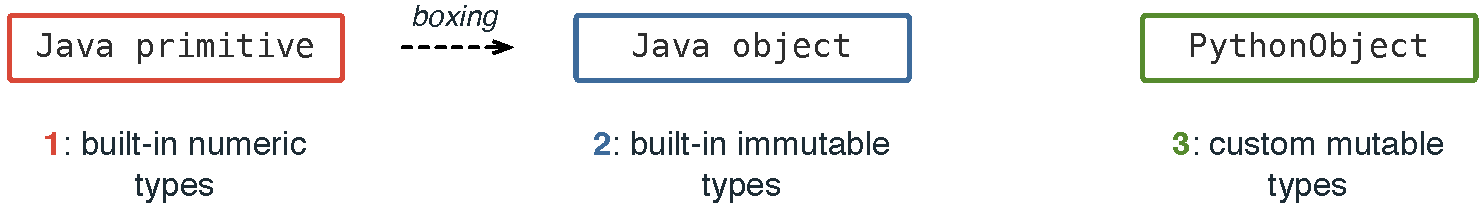
\includegraphics[scale=.6]{figures/ch5-three-data-representations}
\caption{Three data representations for Python objects}
\label{fig:ch5-three-data-representations}
\end{figure}

ZipPy internally uses multiple data representations to model Python objects.
Figure~\ref{fig:ch5-three-data-representations} illustrates this design scheme.
The descriptions of each data representation are as follows:

\begin{enumerate}

\item \textbf{Built-in numeric types}
ZipPy, as explained in Chapter~\ref{sec:ch3-fast-arithmetics}, models some built-in numeric types, like \texttt{bool}, \texttt{int} and \texttt{float}, using Java primitives.
This approach helps to achieve Java level performance for arithmetic operations in ZipPy.
We refer types that has a Java primitive representation as \emph{unboxable}.
Each \emph{unboxable} numeric type in ZipPy has a corresponding \emph{boxed} representation using Java objects as a fallback.
As shown in the Figure, a boxing operation will convert an instance of unboxable type, e.g., \texttt{int}, from its Java primitive representation to the boxed one.

\item \textbf{Built-in immutable types}
Similar to Jython, we implement Python built-in types including numeric types as regular Java classes.
In this way we map Python's built-in type hierarchy onto a Java class based type hierarchy.
Unlike custom types, all built-in types in Python are immutable meaning that user program cannot modify the attributes of an instance of a built-in type.
We take advantage of this immutability by modeling Python built-in types directly using Java classes on the JVM.

\item \textbf{Custom mutable types}
All custom or user defined types in Python are mutable.
That includes Python modules, custom type definitions written in Python and instances of custom classes.
We model them using still a regular Java object, an instance of \texttt{PythonObject} in ZipPy, to circumvent the performance overhead incurred by using a hash map.
ZipPy maps Python attribute accesses to field accesses on the \texttt{PythonObject} object.
We support attribute mutation by maintaining an object layout table for each Python object.
The object layout table keeps track of the memory offset for each attribute that is currently stored on the object.
We will discuss how we support attribute modifications on custom types in more detail in Section~\ref{sec:ch5-custom-mutable-types}.

\end{enumerate}

Although we model Python objects using different physical data representations, our approach preserve the semantics that every data in Python is an object.
ZipPy support object like operations on each of the data representations described above.
What differs our approach to the existing ones is that we do not treat all Python data types in the same way.
We try to pick the most efficient construct offered by the JVM that is suitable for implementing particular types in Python.
To be more specific, modeling Python numbers as Java primitives enables the best arithmetics performance achievable on the JVM.
Using Java object to model Python object brings the opportunity for ZipPy to close the performance gap of object operations between existing implementations of Python and Java.

\subsection{Attribute Resolutions}
\label{sec:ch5-attribute-resolution}

Each object in Python is a collection of key value pairs.
Each key value pair is an attribute of the object with the key being the symbol of the attribute.
The value of an attribute is essentially another Python object.
Like other dynamic languages, Python allows programmers to reference, add or delete attributes on an object.
Attribute referencing follows a rule referred as method resolution order in Python.
Upon the creation of a custom type or class in Python, the interpreter calculates a linearized list of types for the newly created type.
Each type in the list is a super type of the new type.
The method resolution order of the new type refers to the order its super types appear in the linearized list.
Given the method resolution order, an attribute resolution on a Python object follows the following steps:

\begin{enumerate}

\item Lookup the attribute from the object itself.
If it does not exist on the object, continue with the next step.

\item Obtaining the class object of the original object through the \texttt{\_\_class\_\_} attribute of the object.
Lookup the attribute from the class object.
If failed, continue with the next step.

\item Obtaining the bases of the object's class through the \texttt{\_\_bases\_\_} attribute of the class object.
Lookup the bases types in the method resolution order until the attribute is found.
Otherwise, if the interpreter fail to resolve the attribute in the end, it throws an \texttt{AttributeError}.

\end{enumerate}

\begin{figure}
\centering
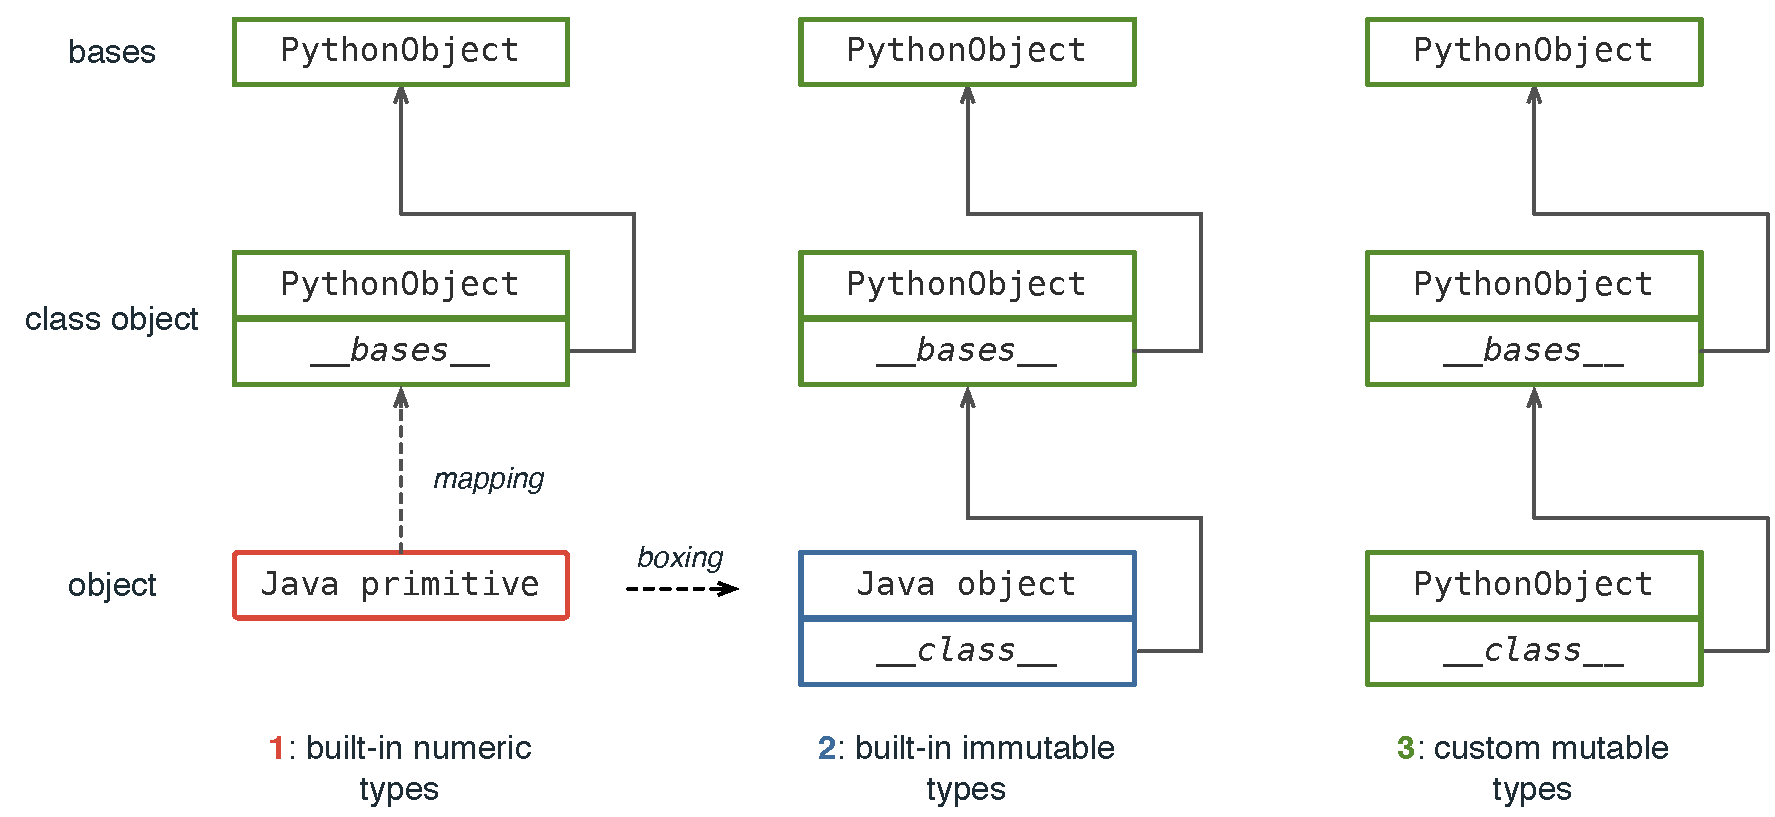
\includegraphics[scale=.54]{figures/ch5-attribute-resolutions}
\caption{Attribute resolution for different data representations}
\label{fig:ch5-attribute-resolutions}
\end{figure}

Since ZipPy uses multiple data representations to model Python objects, we also need to implement the above mentioned attribute resolution differently for each representation.
Figure~\ref{fig:ch5-attribute-resolutions} illustrates this process for the three different data representations used in ZipPy.
For simplicity, we model all class objects using a mutable \texttt{PythonObject}.
Each \texttt{PythonObject} stores the reference to the next node in the lookup chain as a dedicated field (\texttt{\_\_class\_\_} and \texttt{\_\_bases\_\_}).
This choice makes the type hierarchy of mutable objects consistent, since every node on the lookup chain is a \texttt{PythonObject}.
Similarly, built-in types modeled using immutable java objects connect to the rest of the lookup chain also use a reference stored in a dedicated field.
For unboxed built-in types, we uses a preprocessed mapping table to associate the Java class of the primitive type to the class object representing its Python type.
For instance, we model a Python integer, which is an instance of the Python \texttt{int} class, using a Java primitive \texttt{int}.
However, we model the Python \texttt{int} class object itself, which is an instance of the class \texttt{type}, using a mutable Java object.
The mapping table maps the Java class of primitive \texttt{int} to the Python \texttt{int} class object, and thus completes the entire lookup chain for unboxed built-in types.

\subsection{Modeling Custom Mutable Types}
\label{sec:ch5-custom-mutable-types}

\begin{figure}
\centering
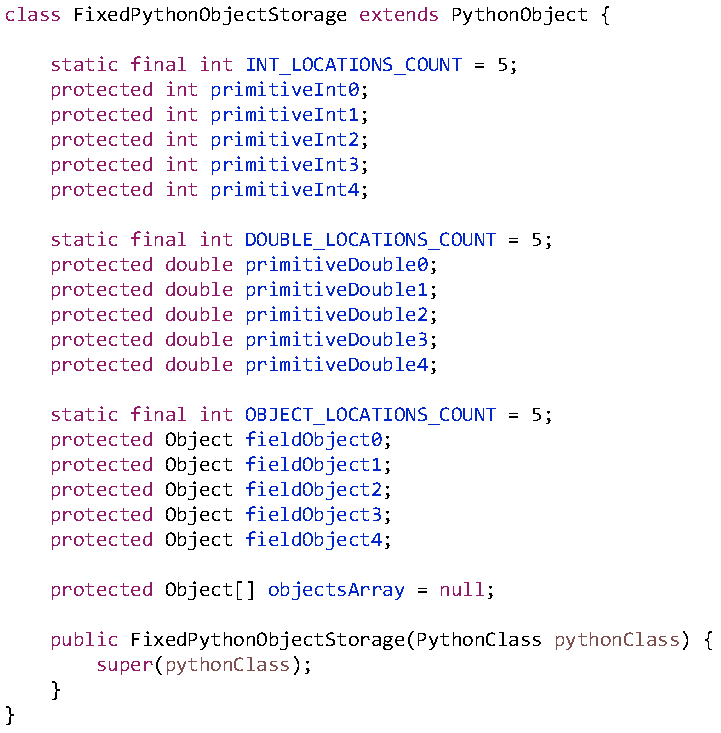
\includegraphics[scale=1.]{figures/ch5-fixed-python-object-code}
\caption{The implementation of \texttt{PythonObject}}
\label{ch5-fixed-python-object-code}
\end{figure}

\begin{figure}
\centering
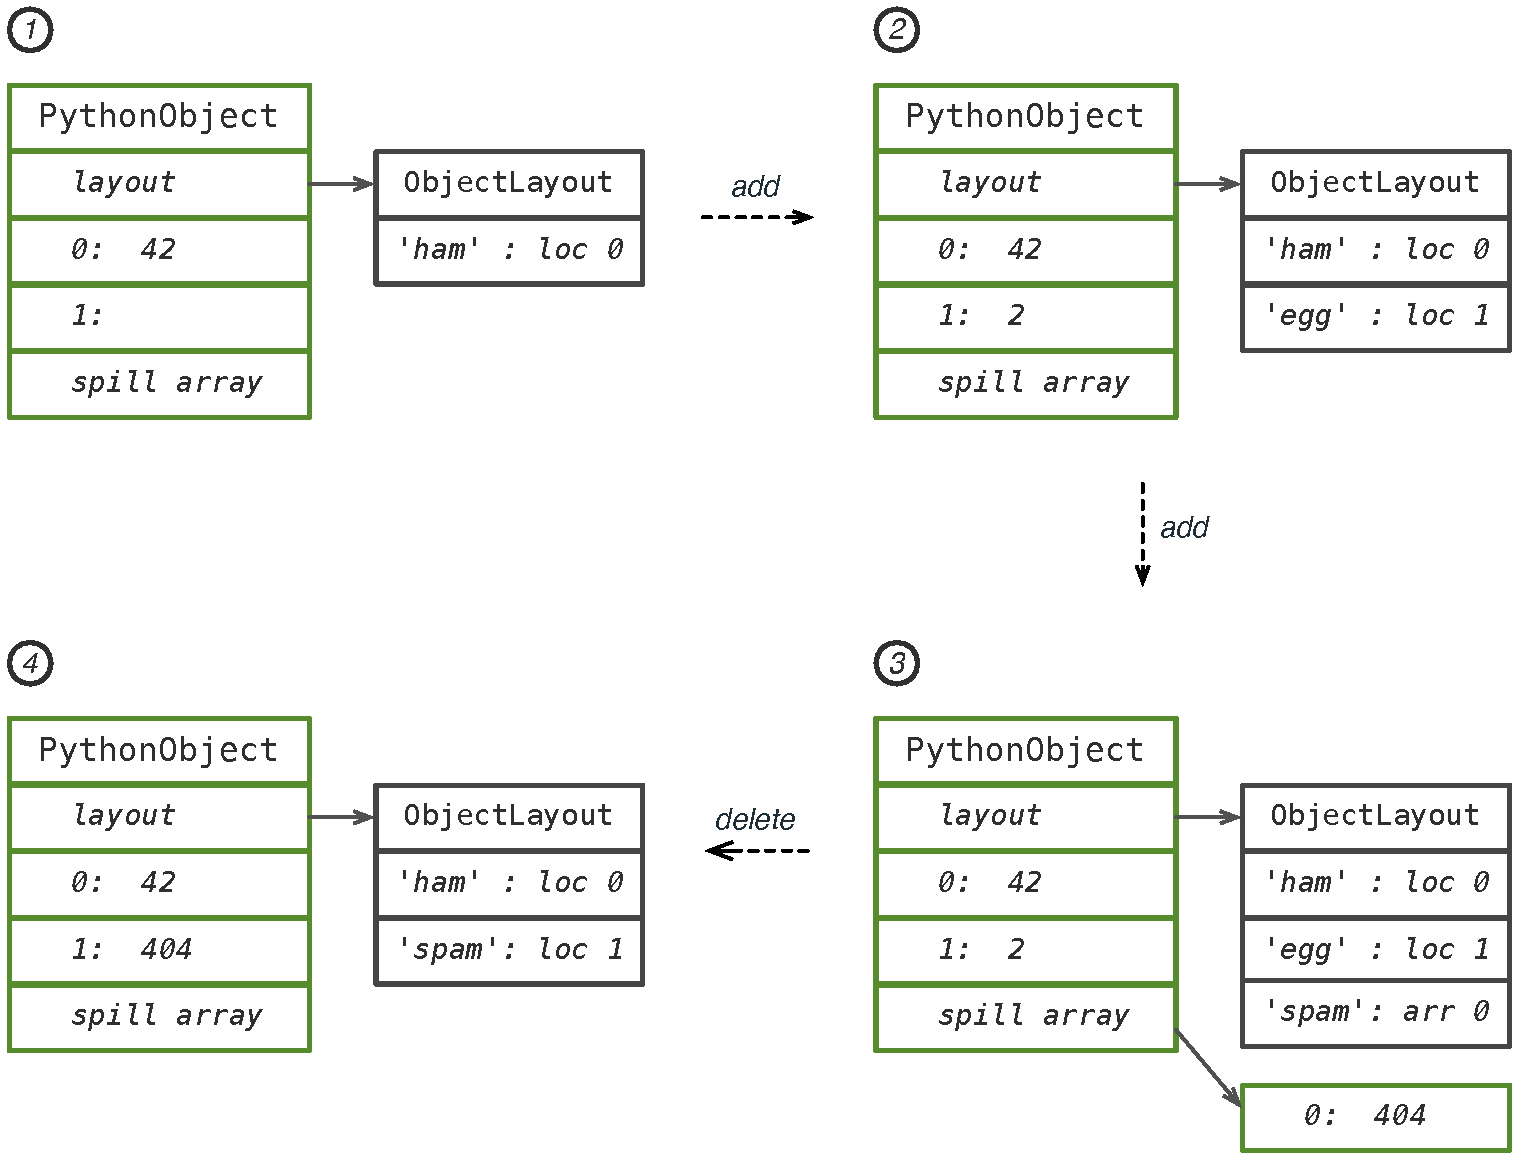
\includegraphics[scale=.6]{figures/ch5-mutable-object-layout-change}
\caption{Mutable object layout}
\label{ch5-mutable-object-layout-change}
\end{figure}

Python allows programmers to add, modify or delete attributes on an object during the execution of the program.
On the other hand, a Java object is fixed.
You can modify the value of a field, but cannot resize or change the layout of an object.
We support this dynamic feature of Python by implementing each Python object using a combination of a fixed \texttt{PythonObject} and a resizable object layout.

Figure~\ref{ch5-fixed-python-object-code} shows an implementation of \texttt{PythonObject} in ZipPy.
Each \texttt{PythonObject} has a fixed number of fields of both primitive and reference types to accommodate its attributes.
Each field on the objec is a \emph{location}.
The object stores each of its attribute on a dedicated \emph{location}.
ZipPy tries to store an unboxed attribute in an unboxed location to avoid the overhead of boxing.
For instance, it tries to store a Java \texttt{int} in an \texttt{int} field when possible.
If all \texttt{int} fields are taken, it tries to stores the attribute in an \emph{boxed} location or an object field.
If no in-object location is available anymore (taken by other attributes), ZipPy will spill the incoming attribute to be stored in the additional object array (field \texttt{objectArray} in Figure~\ref{ch5-fixed-python-object-code}).
The additional object array gives the fixed \texttt{PythonObject} the ability to store more attributes than its own capacity by paying the price of another level of direction and possibly auto-boxing.

An object layout attached to a \texttt{PythonObject} keeps track of the list of attributes stored on the object as well as the location of each attribute.
It is essentially a table that maps the symbol of an attribute to its location.
The table records modifications made dynamically to the attributes of the object.
Figure~\ref{ch5-mutable-object-layout-change} illustrates how this process works by using a hyperthetical Python object.
The layout of the shown object goes through the following stages:

\begin{enumerate}

\item The object initially has one attribute \textsf{ham} stored in location $0$ with the value $42$.

\item After adding the attribute \textsf{egg}, the object now has both \textsf{ham} and \textsf{egg} stored in location $0$ and $1$ respectively.

\item Since both in-object locations are taken, the object stores the new attribute \textsf{spam} in the spill array at the index $0$.
The rest of the layout remain unchanged.

\item The deletion of \textsf{egg} frees location $1$ on the object.
The object reassigns the newly available in-object location to \textsf{spam} to make sure that location assignments are optimal.
It also update the layout table to reflect the new changes.

\end{enumerate}

We simplified the structure of the Python object shown in Figure~\ref{ch5-mutable-object-layout-change} for brevity.
The actual algorithm for a layout update is more complicated.
Adding or deleting an attribute triggers a layout update.
The layout update tries to stores as many unboxed attributes in an unboxed location as possible.
The spill array allocation is lazy so that we only allocate the array when necessary.
During the layout update, ZipPy calculates the size of the addtional spill array needed to accommodate all the attributes.
If it requires a spill array, we conservatively allocate an array that is just enough to store all the attributes.

The type of an attribute can change at runtime.
A type change also triggers a layout update.
Our current solution is to assign a location that matches the most general type of an attribute.
Once an unboxed attribute becomes boxed, we always assign a boxed location for this attribute in the future.

Our approach uses \texttt{PythonObject}s simply as a physical storage for the attributes of a Python object.
We detach the layout description of the Python object from its storage component, which gives us the freedom to customize the behavior of attribute accesses in ZipPy without being restricted by Java's own object model.
Since we model class objects in the same way as regular objects in Python, they enjoy the same potential peformance benefit achieved by this design.

\subsection{Inline Caching for Attribute Accesses}

As explained in Section~\ref{sec:ch5-custom-mutable-types}, the layout table stores the location of each object attribute.
Access an attribute requires looking up its location information from the layout table and then performing a memory operation that reads from or writes to the obtained memory location.
Since we implement the layout table using a hash map, the cost of accessing the table is as expensive as attribute accesses on a hash map based object.
However, ZipPy optimizes attribute accesses by caching attribute locations after a full layout table lookup.
This technique, inspired by previous research on virtual machines~\cite{Deutsch1984, holzle1991, Brunthaler2010inca}, amortizes the cost of accesses to the same attribute on the object of the same type.

\subsubsection{Attribute Access Dispatch Chain}

\begin{figure}
\centering
\subfigure[Structure of \texttt{GetAttributeNode}]{
	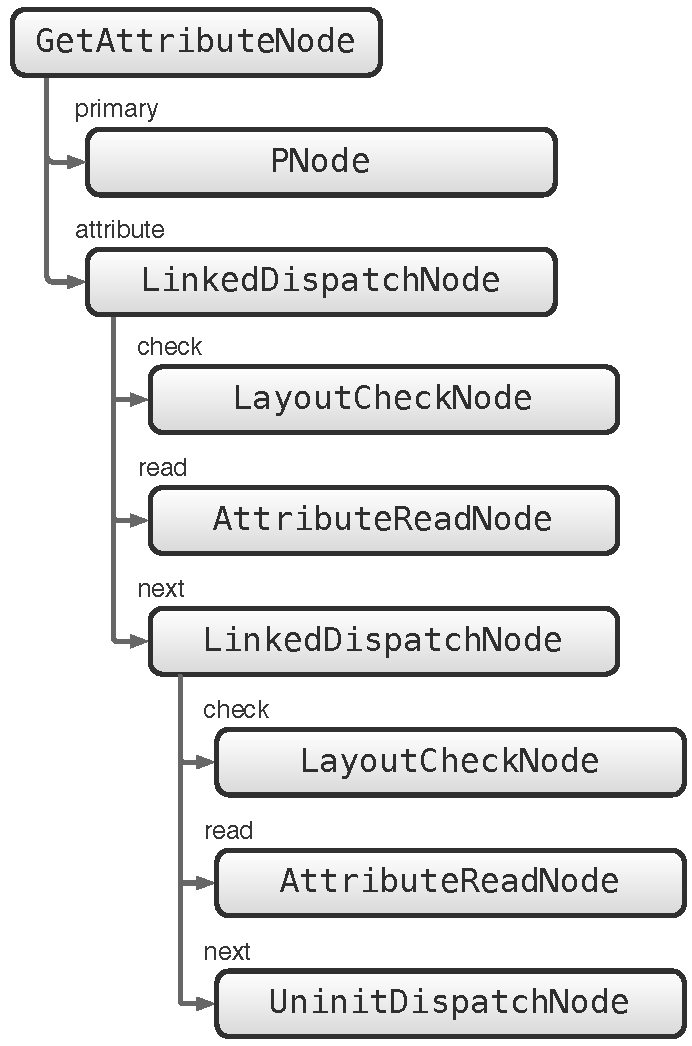
\includegraphics[scale=.55]{figures/ch5-get-attribute-node}
	\label{fig:ch5-get-attribute-node}
}
\subfigure[Structure of \texttt{SetAttributeNode}]{
	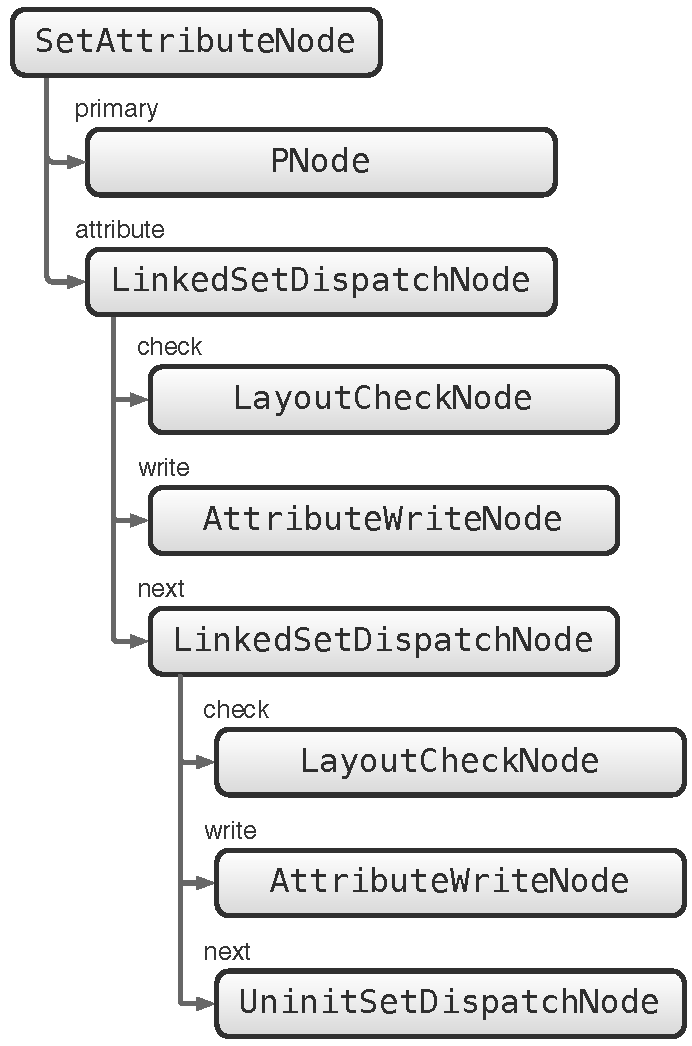
\includegraphics[scale=.55]{figures/ch5-set-attribute-node}
	\label{fig:ch5-set-attribute-node}
}
\caption{Attribute access dispatch chain}
\label{fig:ch5-attribute-access-dispatch-chain}
\end{figure}

Like the other operation, we model attribute accesses using AST nodes in ZipPy.
We model an attribute read operation using a \texttt{GetAttributeNode} and write operation using a \texttt{SetAttributeNode}.
Figure~\ref{fig:ch5-attribute-access-dispatch-chain} illustrates the structure of these two nodes.
In each attribute access node, the \textsf{primary} child node represents the primary expression, the component precedes the period in Python's syntax.
The \textsf{primary} node evaluates to the Python object, on which we perform the attribute access.
The \textsf{attribute} nodes shown in both Figure~\ref{fig:ch5-get-attribute-node} and~\ref{fig:ch5-set-attribute-node} are dispatch chains that perform the actual read or write on the resolved object.

The attribute access dispatch chain is a link list of dispatch nodes.
Each dispatch node has a \textsf{next} field that points to the next dispatch node except for the last one.
The chain forms a polymorphic inline cache with each node working as an individual cache entry.
Each entry stores the object layout and the location of a previously accessed attribute.
Upon a successive access to the attribute on an object having the same layout, the matching dispatch node performs a memory access directly using the cached location.
In other words, a cache hit in the dispatch chain voids executing the slow path lookup on the object layout.

ZipPy performs an attribute access operation in a number of steps.
It first evaluates the primary object, and passes the object to the dispatch chain.
The resolved primary object travels through the dispatch chain from the top to the bottom one dispatch node after another.
Each dispatch node tests the cached object layout against the one of the incoming object.
If the test returns a match, the dispatch node performs a fast read or write on the object and returns the result to the parent node if necessary.
Otherwise, execution falls to the next dispatch node on the chain until a cache hit occurs.
If no cache hit happened, the primary object reaches the uninitialized dispatch node at the end of the chain.
The unitialized dispatch node, in this case, performs a full attribute access on the primary object including a lookup on its layout table.
Additionally, it also constructs a new cached dispatch node and inserts the new node between the unitialized dispatch node and its predecessor.
The added entry increases the depth of the inline cache as well as the chance of a cache hit in the future.
However, if the cache depth reaches a certain threshold, ZipPy rewrites the entire dispatch chain to a single generic dispatch node that always perform a slow path lookup.

Each cache entry in the dispatch chain consists of a cluster of nodes coordinated by the dispatch node.
Besides the \textsf{next} field pointing to the next node, each dispatch node has a \texttt{LayoutCheckNode} as well as a \texttt{AttributeReadNode} or \texttt{AttributeWriteNode} (Figure~\ref{fig:ch5-attribute-access-dispatch-chain}).
The \textsf{check} node stores the cached object layout and performs the layout test.
The \textsf{read} or \textsf{write} node stores the cached attribute location and performs the actual read or write on the primary object.
When a layout update happens, ZipPy creates a new layout instance for the associated Python object.
ZipPy also signals the old layout as invalid, since it does not describe a valid layout for the associated object anymore.
Therefore, when performing a layout test the \texttt{LayoutCheckNode} also checks the validity of the cached layout.
If the cached layout become invalid, it throws an exception back to the parent node.
ZipPy handles the exception by remove the invalid cache entry from the dispatch chain.

\subsubsection{Dispatch Node Transformation}

\begin{figure}
\centering
\includegraphics[scale=.65]{figures/ch5-attribute-dispatch-transformation}
\caption{The transformation of a get attribute dispatch node}
\label{fig:ch5-attribute-dispatch-transformation}
\end{figure}

The above mentioned attribute access dispatch chain initially starts with a single uninitialized dispatch node.
It expands into a chain linking a number of \texttt{LinkedDispatchNode} during execution.
If the depth of the chain overflows a given limit, the entire chain transforms to a \texttt{GenericDispatchNode}.
Figure~\ref{fig:ch5-attribute-dispatch-transformation} further illustrates this transformation.
The descriptions of the transformation rules depicted in the Figure are as follows:

\begin{enumerate}

\item Upon a successful specialization, the uninitialized dispatch node produces a specialized dispatch node that caches the layout of the primary object and the location of the attribute being accessed.
Depending on the data representation of the primary object, it chooses the \texttt{LinkedDispatchUnboxNode} as the transformation target to avoid auto-boxing.
A \texttt{LinkedDispatchUnboxNode} stores the Java class of the \emph{unboxed} object.

\item A \texttt{LinkedDispatchBoxedNode} performs the layout test through an identify check between the cached layout and the layout of the incoming primary object.
A layout test on a \texttt{LinkedDispatchUnboxedNode} compares the cached Java class to that of the primary object.
If the layout test returns a match, the cached dispatch node remains unchanged.
Note that in an attribute read operation, as explained in Section~\ref{sec:ch5-attribute-resolution}, the resolved attribute may not be stored on the primary object itself.
In fact, the actual owner can be any object on the attribute resolution chain of the primary object.
In this case, the cached dispatch node needs to conservatively cache all the layout of the objects on the attribute resolution chain from the primary object itself upto the owner of the resolved attribute.
In the layout test, the dispatch node needs to perform a series of checks to ensure the validity of the cache layouts.

\item If the layout test returns a miss match or a cache miss occurs, the cached dispatch node redirects execution to the next node on the dispatch chain.
The same rules apply to the transformation of the next dispatch node.
In addition, if the cached layout become invalid, ZipPy removes the dispatch node from the chain.

\item If the execution of an attribute access dispatch reaches an uninitialized dispatch node and the depth of the chain has reached a certain threshold,
the dispatch node replaces the entire dispatch chain with a \texttt{GenericDispatchNode}.
A \texttt{GenericDispatchNode} is stable meaning that it always perform a slow path attribute lookup and does not re-specialize to other nodes.

\end{enumerate}

The deeper the dispatch chain the more step it takes to reach the bottom portion of the chain.
The cost of hitting a cache entry located close to the bottom of the chain grows with the depth of the chain.
Thus, it is not cost effective to grow the dispatch chain indefinitely.
On the other hand, for a program location exhibits a high degree of polymorphism or also referred as a megamorphic dispatch site,
optimizing for just a few number of cases only affects a limited fraction of the overall execution occurred at this program location.
An optimization strategy like inline caching is unlikely to have an substantial performance impact in this case.
In summary, for a megamorphic dispatch site using a generic dispatch node is simpler and as efficient as forming a deep dispatch chain.

\section{Call Site Modeling}

In general you can call any \emph{callable} object in Python.
Making a call in different contexts has different semantics allowing the caller to pass arguments to the callee in different ways.

\subsection{Call Sites Structures in Python}
\label{sec:ch5-structure-of-call-sites}

\begin{figure}
\centering
\subfigure[Simple call site]{
	\includegraphics[scale=.9]{figures/ch5-call-site-simple-code}
	\label{fig:ch5-call-site-simple-code}
}
\subfigure[Attribute call site]{
	\includegraphics[scale=.9]{figures/ch5-call-site-attribute-code}
	\label{fig:ch5-call-site-attribute-code}
}
\caption{Two types of calls in Python}
\label{fig:ch5-call-site-synteax-code}
\end{figure}

Figure~\ref{fig:ch5-call-site-simple-code} shows the syntax of a simple call in Python.
It is simple enough for us to explain the basic steps of making a call in Python without getting into more complicated details.
The execution of the call shown in the Figure involves the following steps.
As the first step, the program needs to look up the symbol \texttt{foo} from the current scope or its enclosing scope with respect to Python's scoping rules.
After resolving the symbol \texttt{foo}, the program then checks the type of the resolved object to determine the eligibility of such call.
Lastly, the actual call takes place using a calling convention that matches the type of the callee object.
The Python interpreter uses different calling convention or passes the arguments to the callee in a different way depending on the actual type of the callee.
For instance, if the callee is a Python class object, the interpreter creates an empty Python object and passes it to the callee as the first argument.

The call site shown in Figure~\ref{fig:ch5-call-site-simple-code} is in its simplest form.
We refer it as a \emph{simple call site}.
The callee resolution for the call shown in Figure~\ref{fig:ch5-call-site-attribute-code} involves an attribute referencing on the Python object \texttt{p}.
We refer this type of call sites as \emph{attribute call sites}, since the actual callee is an attribute of the primary object like \texttt{p} in the Figure.
The primary object, however, can be any namespace backed by a Python object such as a regular object, a class object or a module.
Looking back at the simple call site as shown in Figure~\ref{fig:ch5-call-site-simple-code},
it is worth noting that the callee resolution might involve an attributing referencing as well depending on the type of the scope in which the call takes place.
For example, if program resolves \texttt{foo} as a global variable, the look up of \texttt{foo} includes an implicit attribute referencing on the current Python module.
Similarly, in a class scope, a simple call to an existing class attribute also involves an implicit attribute look up on the enclosing class object.
% say something about motivates the structure of the AST
The same syntax implies different semantics and ways to make the actual call at runtime.
To capture this variation, we decompose a call site in Python into multiple components and assemble them in different ways to serve different variations.
This way allows us to apply specializations on each component separately to accelerate calls in Python programs.

\subsubsection{The AST of Call Sites}

\begin{figure}
\centering
\includegraphics[scale=.5]{figures/ch5-python-call-node-basic}
\caption{The structure of a \texttt{PythonCallNode}}
\label{fig:ch5-python-call-node-basic}
\end{figure}

Figure~\ref{fig:ch5-python-call-node-basic} illustrates the basic structure of a call node in ZipPy.
A \texttt{PythonCallNode} employees five child nodes representing five components of the call site.
Each child node can further expand into its own sub tree depending on the complexity of the component.
A call node performs a Python call in-coorperating its child nodes in the following steps:

\begin{enumerate}

\item The primary node evaluates the primary object of the call.
If the primary component is missing, the primary node returns the constant Python \texttt{None} object.

\item The callee node resolves the actual callee object using the previously resolved primary object if necessary.
If the callee resolution does not involve an attribute referencing, it ignores the primary object.

\item The arguments node evaluates all the arguments, and returns them to the call node as a Java array.

\item The keywords node evaluates all the keyword arguments, and returns them to the call node in an Java array.

\item The \texttt{PythonCallNode} passes the evaluated primary object, callee, arguments array and keyword arguments array to the dispatch node.
The dispatch node performs the actual call using an inline caching inspired dispatch chain scheme~\cite{Deutsch1984, holzle1991}, and passes all the arguments to the AST of the callee.
We will explain the call dispatch nodes in more detail in Section~\ref{sec:ch5-call-site-caching-and-inlining}.

\end{enumerate}

Note that some components like the primary or keyword arguments are not always present.
In case that an optional component is missing, we still model it as a dummy node that returns a \texttt{None} or an empty Java array to make it consistent for all call nodes.
The \texttt{PythonCallNode} organizes different components of the call site and handles transformations like type specialization and de-optimization at runtime.

\subsection{Call Node Specializations}

Similar to the type specializations of arithmetics as we discussed in Chapter~\ref{chp:ch3-zippy}, ZipPy applies specializations to call nodes against the type of the callee through node rewriting.
The interpreter initially constructs a call node using the uninitialized version (\texttt{UninitCallNode} in Figure~\ref{fig:ch5-call-node-specialization-simple}).
Upon the first execution of the call, the uninitialized call node uses a slow path to resolve the primary object and callee.
At the same time, it rewrites itself to a derivative version that is tailored to the resolved primary and callee.
Not only that the call node specializes itself, it also applies type specializations to its child nodes during the rewriting process.
In this Section, we explain how ZipPy applies call node specializations for different call sites and callee types.

\subsubsection{Specialization for Simple Call Sites}

\begin{figure}
\centering
\includegraphics[scale=.5]{figures/ch5-call-node-specialization-simple}
\caption{Call node specializations for a simple call site}
\label{fig:ch5-call-node-specialization-simple}
\end{figure}

As explained in Section~\ref{sec:ch5-structure-of-call-sites}, the callee resolution of a simple call site (Figure~\ref{fig:ch5-call-site-simple-code}) depends on the type of the namespace to which the callee belongs.
Therefore, the specialization of a simple call site needs to cover different resolution cases.
Figure~\ref{fig:ch5-call-node-specialization-simple} illustrates various call node transformations of a simple call site.
The description of the three different specialization cases shown in the Figure is as follows:

\begin{enumerate}

\item \textbf{Callee in function activation}
The call takes place in a function scope.
The resolved callee is a variable of the function's lexical scope or its enclosing scope.
The primary object does not exist or is \texttt{None} in this case.
Therefore, the primary node is an \texttt{EmptyNode} that returns an \texttt{None}.
The callee nodes retrieve the callee object from the function's activation or the frame object as discussed in Chapter~\ref{sec:ch4-frame-and-control}.
Although type specialization is also applicable to the \texttt{ReadLocalVariableNode}, given that the callee is guarantee to be a boxed object, type specialization in this case has limited benefit.
However, Truffle is still able to optimize frame accesses by eliminating heap allocation of the frame object when applicable.

\item \textbf{Callee as a module attribute}
The resolved callee is an attribute of a module, e.g., the global scope of the current module or the built-in module.
The retrieval of the callee in this case involves an implicit attribute referencing on the primary module object.
Since the primary object is boxed, ZipPy specializes the call node to a \texttt{BoxedCallNode}.
The primary node is a wrapper node that holds a reference to the current module object.
The callee node reads the callee attribute from the module object returned by the primary node.
The \texttt{ReadGlobalNode} accesses the built-in module if it failed to resolve it from the global scope module.
Upon a successful resolution of the callee object, the \texttt{ReadGlobalNode} caches the actual primary object.
For instance, if the resolved callee object is an attribute of the built-in object, the node caches the built-in object instead of the current module.
Caching speedups subsequent attribute accesses by accessing the cached object directly as long as the attributes of the object remain unchanged.

\item \textbf{Callee as a class attribute}
The call takes place in a class scope.
The resolved callee is an existing class attribute of the enclosing scope.
Class definition works as a special function in Python.
The evaluation of the class definition statement is essentially a call to the special function.
The interpreter passes an empty class object as the first argument to the function, and the class definition function populates the class object with attributes like functions.
The call to the class definition function returns the created class object containing attributes specified by in the class definition.
To access an existing attribute of the defining class, we need to first retrieve the defining class object.
The \texttt{ReadArgumentNode} does so by reading the argument array passed by the caller of the class definition.
the callee node then reads the callee attribute from the primary class object.
The \texttt{GetAttributeNode} also enjoys type specialization and caching on its own, which we will discuss more in Section~\ref{sec:ch5-object-module}.

\end{enumerate}

The call node specializations illustrated in Figure~\ref{fig:ch5-call-node-specialization-simple} are based on the resolution of the primary object and callee.
We simplified the Figure to not show the arguments node and the keyword arguments node, since their specialization are orthogonal callee resolutions.

\subsubsection{Specialization for Attribute Call Sites}

\begin{figure}
\centering
\subfigure[Boxed primary]{
	\includegraphics[scale=.7]{figures/ch5-attribute-call-site-boxed-code}
	\label{fig:ch5-attribute-call-site-boxed-code}
}
\subfigure[Unboxed primary]{
	\includegraphics[scale=.7]{figures/ch5-attribute-call-site-unboxed-code}
	\label{fig:ch5-attribute-call-site-unboxed-code}
}
\caption{Attribute call sites with different primary object representations}
\label{fig:ch5-attribute-call-site-boxed-unboxed-code}
\end{figure}

In Chapter~\ref{sec:ch5-object-module} we discussed that ZipPy models Python objects using multiple data representations to make arithmetics and data accesses more efficient.
Since the physical data representation of Python objects differs in ZipPy, attribute lookups on objects backed by different representations are also different.
Figure~\ref{fig:ch5-attribute-call-site-boxed-unboxed-code} shows two attribute call sites.
The primary object of the left one, \texttt{h}, is a user custom Python object (Figure~\ref{fig:ch5-attribute-call-site-boxed-code}).
The primary object \texttt{n} in the one shown in Figure~\ref{fig:ch5-attribute-call-site-unboxed-code} is a built-in integer.
In ZipPy, we model custom objects using a boxed Java object, and map an attribute access to the Python object to a field access on the Java object.
On the other hand, ZipPy represents Python integers and some other built-in data types as Java primitives.
% probably did not explain it very clearly....
Therefore, attribute lookup on those built-in types involves a mapping that associates the instance of the type to the meta class object of the type containing the target attribute.

\begin{figure}
\centering
\includegraphics[scale=.5]{figures/ch5-call-node-specialization-attribute}
\caption{Call node specializations for an attribute call site}
\label{fig:ch5-call-node-specialization-attribute}
\end{figure}


% the specializations shown above covers the majority of calls in Python.
% However, they are not meant to be comprehensive. there are corner cases that we do not cover in this thesis due to space limitations.
% call node specialization captures the fast path of callee resolution.....
% the next chapter will talk about how we further optimize calls in Python.

\subsection{Call Site Caching and Inlining}
\label{sec:ch5-call-site-caching-and-inlining}

\subsection{Inline Caching Based Call Dispatching}

\subsection{Call Inlining in Truffle}

\chapter{Evaluation}
\label{chp:ch5-evaluation}

To fully evaluate the effectiveness of the optimizations we discussed in the Chapter~\ref{chp:ch3-zippy}, Chapter~\ref{chp:ch4-peeling} and Chapter~\ref{chp:ch5-object}, we evaluate the performance of ZipPy in the following steps:
First we evaluate the overall performance of ZipPy by running a selection of conventional benchmarks.
These benchmarks are popular among the virtual machine research and Python communities.
They provide a good indication of the overall performance of a programming language implementation.
Second we examine the effectiveness of generator peeling using a set of real world and generator intensive Python programs.
As the last step, we analyze the performance and space impact of using flexible object storage generation in ZipPy.
We organize our extensive performance experiments by comparing ZipPy with the existing Python VMs.

\section{The Performance of ZipPy}
\label{sec:ch6-performance-of-zippy}

\subsection{Experiment Setup}

We evaluate the overall performance of ZipPy by comparing the performance of our system with existing Python VMs, such as CPython~\cite{python}, Jython~\cite{jython} and PyPy~\cite{pypy}.
Our system setup is as follows:

\begin{itemize}

\item Intel Xeon E5462 Quad-Core processor running at a frequency of 2.8GHz, on Mac OS X version 10.9.3 build 13D65.

\item Apple LLVM 5.1, OpenJDK 1.8.0\_05, Truffle/Graal 0.3.\footnote{From source code repository \url{http://hg.openjdk.java.net/graal/graal}}

\end{itemize}

The VM versions used in the comparison and the description of their execution models are as follows:

\begin{itemize}

\item CPython 2.7.6 and 3.4.0: Interpreter only.

\item Jython 2.7-beta2:
Python 2 compliant, hosted on JVMs.
Compiles Python modules to Java classes and lets the JVM JIT compiler further compiles them to machine code.

\item PyPy 2.3.1 and PyPy3 2.3.1: Python 2 and 3 compliant respectively.
Uses a meta-tracing JIT compiler that compiles Python code to machine code.

\end{itemize}

% Python 2 vs. Python 3
Python 3 is not backward compatible with Python 2.
Although ZipPy exclusively supports Python 3, including well-established Python 2 VMs in the comparison highlights the potential of our optimization.
The benchmarks we chose support both Python 2 and 3.
The same code, however, suffers from a slight difference in the semantics interpreted by different VMs.

% how we measure, peak performance
We run each benchmark ten times on each VM and average the execution times.
For VMs that use a tiered execution strategy, we warm up the benchmarks to ensure that the code is just-in-time compiled.
This allows us to properly measure peak performance.

\subsection{Benchmark Selection}

\begin{table*}
  \begin{center}
    \begin{tabular}{ l l }
    \toprule
    Benchmark suite & Included benchmarks \\
    \midrule
	Computer Language Benchmarks - & \textsf{binarytrees}, \textsf{fannkuchredux}, \textsf{fasta}, \textsf{mandelbrot}, \textsf{meteor} \\
	Games & \textsf{nbody}, \textsf{pidigits}, \textsf{spectralnorm} \\
	\midrule
	Unladen Swallow Benchmarks &  \textsf{float}, \textsf{richards} \\
	\midrule
	PyPy Benchmarks & \textsf{chaos}, \textsf{deltablue}, \textsf{go} \\
    \bottomrule
	\end{tabular}
    \caption{Benchmarks selection}
    \label{tab:ch6-regular-benchmark-selection}
  \end{center}
\end{table*}

We selected a number of benchmarks for the performance experiments from three popular benchmark suites.
The descriptions of the chosen benchmark suites are as follows:

\begin{itemize}

\item Computer Language Benchmarks Game~\cite{benchmarkgame}: a popular benchmark suite for evaluating and comparing the performance of different programming languages.

\item Unladen Swallow Benchmarks~\cite{unladen.swallow}: the benchmark suite used by the unladen swallow project.
Unladen swallow is an optimization branch of CPython built by Google.
The goal of the project was to become a faster yet fully compatible modification of CPython.
Its benchmark suite is well-regarded in the Python community.

\item PyPy Benchmarks: a collection of benchmarks used by the PyPy project.

\end{itemize}

Table~\ref{tab:ch6-regular-benchmark-selection} summerizes the benchmarks we selected in this experiment from the above mentioned suites.
Since we focus on the overall performance of Python VMs, we intentionally leave out benchmarks that are sentitive to the performance of generators.
We selected benchmarks that are written in both imperative and object oriented styles.

\subsection{Experiment Results}

\begin{table*}
  \small
  \begin{center}
  \begin{tabular}{ l r r r r r r }
  \toprule
  Benchmark     & CPython3  & CPython  & Jython  & PyPy     & PyPy3    & ZipPy \\
  \midrule
  \textsf{binarytrees}   & $5.40$    & $5.10$   & $10.76$ & $14.05$  & $14.60$  & $39.49$ \\
  \textsf{fannkuchredux} & $2.27$    & $2.20$   & $1.17$  & $101.24$ & $107.52$ & $198.94$ \\
  \textsf{fasta}         & $15.52$   & $16.20$  & $24.13$ & $182.09$ & $174.55$ & $241.76$ \\
  \textsf{mandelbrot}    & $9.00$    & $9.70$   & $3.03$  & $98.15$  & $97.35$  & $105.18$ \\
  \textsf{meteor}        & $100.55$  & $102.83$ & $77.14$ & $265.43$ & $263.75$ & $213.77$ \\
  \textsf{nbody}         & $10.12$   & $9.87$   & $7.40$  & $122.83$ & $122.07$ & $62.42$ \\
  \textsf{pidigits}      & $77.02$   & $77.40$  & $47.59$ & $75.25$  & $73.02$  & $46.59$ \\
  \textsf{spectralnorm}  & $0.90$    & $1.20$   & $1.70$  & $114.60$ & $114.52$ & $115.29$ \\
  \textsf{float}         & $10.82$   & $10.23$  & $11.37$ & $93.57$  & $93.82$  & $191.68$ \\
  \textsf{richards}      & $16.77$   & $15.83$  & $20.35$ & $495.38$ & $490.70$ & $840.93$ \\
  \textsf{chaos}         & $2.05$    & $2.40$   & $3.17$  & $83.77$  & $52.65$  & $139.94$ \\
  \textsf{deltablue}     & $19.62$   & $16.77$  & $26.19$ & $590.25$ & $571.82$ & $460.37$ \\
  \textsf{go}            & $23.15$   & $24.97$  & $46.16$ & $157.29$ & $154.07$ & $356.80$ \\
  \bottomrule
  \end{tabular}
  \caption{The scores of Python VMs running regular benchmarks}
  \label{tab:ch6-regular-benchmarks-scores}
  \end{center}
\end{table*}

\begin{table*}
  \small
  \begin{center}
  \begin{tabular}{ l r r r r r r }
  \toprule
  Benchmark     & CPython3  & CPython  & Jython  & PyPy     & PyPy3    & ZipPy \\
  \midrule
  \textsf{binarytrees}   & $1.00$    & $0.94$   & $1.99$  & $2.60$   & $2.70$   & $7.31$ \\
  \textsf{fannkuchredux} & $1.00$    & $0.97$   & $0.51$  & $44.53$  & $47.29$  & $87.50$ \\
  \textsf{fasta}         & $1.00$    & $1.04$   & $1.55$  & $11.73$  & $11.24$  & $15.57$ \\
  \textsf{mandelbrot}    & $1.00$    & $1.08$   & $0.34$  & $10.91$  & $10.82$  & $11.69$ \\
  \textsf{meteor}        & $1.00$    & $1.02$   & $0.77$  & $2.64$   & $2.62$   & $2.13$ \\
  \textsf{nbody}         & $1.00$    & $0.97$   & $0.73$  & $12.13$  & $12.06$  & $6.17$ \\
  \textsf{pidigits}      & $1.00$    & $1.00$   & $0.62$  & $0.98$   & $0.95$   & $0.60$ \\
  \textsf{spectralnorm}  & $1.00$    & $1.33$   & $1.89$  & $127.33$ & $127.25$ & $128.10$ \\
  \textsf{float}         & $1.00$    & $0.95$   & $1.05$  & $8.64$   & $8.67$   & $17.71$ \\
  \textsf{richards}      & $1.00$    & $0.94$   & $1.21$  & $29.53$  & $29.25$  & $50.13$ \\
  \textsf{chaos}         & $1.00$    & $1.17$   & $1.55$  & $40.88$  & $25.69$  & $68.28$ \\
  \textsf{deltablue}     & $1.00$    & $0.85$   & $1.33$  & $30.08$  & $29.14$  & $23.46$ \\
  \textsf{go}            & $1.00$    & $1.08$   & $1.99$  & $6.79$   & $6.66$   & $15.41$ \\
  \textbf{mean}          & \textbf{1.00}    & \textbf{1.02}   & \textbf{1.05}  & \textbf{12.15}  & \textbf{11.68}  & \textbf{15.34} \\
  \bottomrule
  \end{tabular}
  \caption{The speedups of Python VMs normalized to CPython3 running regular benchmarks}
  \label{tab:ch6-regular-benchmarks-speedups}
  \end{center}
\end{table*}

Table~\ref{tab:ch6-regular-benchmarks-scores} and~\ref{tab:ch6-regular-benchmarks-speedups} shows the results of our experiments.
We use a score system to gauge VM performance.
We calculate the score by dividing $1000$ by the execution time of the benchmark.
A score system is more intuitive than execution times for visualization purpose.
It also offers a higher resolution for our performance measurements.
We carefully chose the program inputs such that the resulting scores stay in the range between $10$ and $1000$.
Larger inputs have limited impacts on the speedups our of optimization.

Table~\ref{tab:ch6-regular-benchmarks-scores} shows the average scores of each Python VM running the selected benchmarks.
Table~\ref{tab:ch6-regular-benchmarks-speedups} shows the average speedups of each VM against CPython3.
We calculate the speedups by normalizing the scores of each VM shown in Table~\ref{tab:ch6-regular-benchmarks-scores} against that of CPython3.
The last row of Table~\ref{tab:ch6-regular-benchmarks-speedups} shows the geometric mean of the speedups of each Python VM relative to CPython3.
As shown in the Table, the average speedup of ZipPy over CPython3 is $\zippyToCPythonRegular{}\times$ with the highest speedup over $128\times$ on \textsf{spectralnorm}.
Note that the performance of ZipPy running the selected benchmarks is even higher than PyPy by around $26\%$

\subsection{Performance Analysis}

The majority of the high number speedups of ZipPy comes from compute intensive benchmarks like the ones from the Computer Language Benchmarks Game.
The unboxed data representation of numeric types in ZipPy successfully optimizes these benchmarks without ever having to go to the boxed representation.
At peak performance, ZipPy executes the entire benchmark by only using Java primitives for arithmetic operations.
This approach effectively enables low level optimizations offered by the underlying Graal compiler, which consequently achieved Java like arithmetics performance for Python programs in our experiments.
Being able to speculatively bring the cost of arithmetic operations in Python much closer to the one in Java is the key distinguisher between ZipPy and the existing JVM-based Python implementations.

The noticeable slow down in \textsf{pidigits} is caused by integer overflows in Python.
After an integer overflow, ZipPy uses a JDK \texttt{BigInteger}~\cite{hotspot} to model integers of a large value.
However, the implementation of \texttt{BigInteger} in the JDK did not outperform the implementation of \texttt{PyInt} in CPython on our benchmark.
We did not pursue in the direction of replacing \texttt{BigInteger} with a more efficient alternative written in Java, since we consider the implementation details of an unbound integer type to be orthogonal to the research we discuss in this thesis.

We also see speedups of multiple of $10\times$ on object-bound benchmarks like \textsf{richards} and \textsf{chaos}.
We only use fixed object storages in this experiment.
The results suggest that the Python object model used in ZipPy is orders of magnitude more efficient that the hash map based ones used in CPython and Jython.
The object layout based approach in ZipPy clears the way on letting the underlying Java compiler to optimize Python object accesses the same way as it does to Java objects.
In the common case where the object layouts stabilize shortly after warming up, ZipPy essentially delivers Java like performance on Python object operations in our experiment.

Overall ZipPy outperforms PyPy in our experiment.
We attribute this advancement to Graal, the underlying Java JIT compiler.
PyPy uses a relatively straight forward tracing JIT compiler to compile Python programs down to machine code.
Whereas Graal is a substantially more sophisticated and aggressive method JIT.
The kinds of optimizations implemented in Graal outnumbered that in PyPy.
Overall we do expect Graal to generate more efficient machine code that the compiler in PyPy.

In general the speedups we achieved in our experiment are inline with other efficient Truffle language implementations~\fxnote{cite other truffle langs?}.
A number of semi built-in optimizations offered by Truffle helped us achieving this result.
The most important ones includes: frame optimization that eliminates the heap allocation of a frame object and Truffle AST inlining.
Another advantage of using Truffle as the base of ZipPy is that it makes it easy for guest language implementers to fine tune the machine code size produced by the compiler.
It offers utilities that helps us to precisely specify the boundary of a JIT compilation rather than fully relying on the compiler heuristics.
This features allows us to carve out less important code paths from the compiled code to make the machine code size more compact.
In summary, by making better use of Truffle ZipPy is able to achieve high speedups when compared with existing Python VMs with low implementation cost.

\section{The Effectiveness of Generator Peeling}

We evaluate the performance of our generator peeling implementation in ZipPy by running Python programs that have intense use of generators.
We used the same experiment setup as we did in the overall performance evaluation of ZipPy in Section~\ref{sec:ch6-performance-of-zippy}.

\subsection{Benchmark Selection}

% benchmark selection
We analyzed hundreds of programs listed on the Python Package Index~\cite{pypi}.
We picked a set of programs that includes compute intensive benchmarks as well as larger applications.
The following chosen programs use generators to various degrees:

\begin{itemize}

\item \textsf{nqueens} is a brute force N-queens solver selected from the Unladen Swallow benchmark suite~\cite{unladen.swallow}.

\item The publicly available solutions to the first $50$ Project Euler problems~\cite{projecteuler}:
\textsf{euler11} computes the greatest product of four adjacent numbers in the same direction in a matrix;
\textsf{euler31} calculates the combinations of English currency denominations.

\item Python Algorithms and Data Structures (PADS) library~\cite{pads}:
\textsf{eratos} implements a space-efficient version of sieve of Eratosthenes;
\textsf{lyndon} generates Lyndon words over an s-symbol alphabet;
\textsf{partitions} performs integer partitions in reverse lexicographic order.

\item \textsf{pymaging} is a pure Python imaging library.
The benchmark draws a number of geometric shapes on a canvas.

\item \textsf{python-graph} is a pure Python graph library.
The benchmark processes a deep graph.

\item \textsf{simplejson} is a simple, fast JSON library.
The benchmark encodes Python data structures into JSON strings.

\item \textsf{sympy} is a Python library for symbolic mathematics.
The benchmark performs generic unifications on expression trees.

\item \textsf{whoosh} is a text indexing and searching library.
The benchmark performs a sequence of matching operations.

\end{itemize}

We learned from our generator survey that popular HTML template engines written in Python use generators.
There are two reasons we do not include them in our performance evaluation.
First, we implement ZipPy from scratch.
It is infeasible for us to support all Python standard libraries required to run these applications.
Second, many of these applications are not compute intensive.
They spent most of the execution time processing Unicode strings or in native libraries, which is not a good indicator of the VM performance.

\subsection{Experiment Results}

\begin{table*}
  \begin{center}
    \begin{tabular}{ l r r r r r r }
      \toprule
      Benchmark             & Score $-$GP & Score $+$GP & Speedup        & No. gen & No. genexp & No. of lines \\
      \midrule
      \textsf{nqueens}      &  $69.09$    & $313.14$    & \textbf{4.53}  & 2/2 & 5/5 & $41$ \\
      \textsf{euler11}      &  $71.42$    & $941.73$    & \textbf{13.19} & 2/2 & 5/5 & $61$ \\
      \textsf{euler31}      &  $47.70$    & $134.35$    & \textbf{2.82}  & 1/1\textsuperscript{\textdagger} & 2/2 & $46$ \\
      \textsf{eratos}       &  $277.13$   & $316.64$    & \textbf{1.14}  & 2/2 & 0/0 & $86$ \\
      \textsf{lyndon}       &  $37.89$    & $859.91$    & \textbf{22.69} & 3/3 & 0/0 & $127$ \\
      \textsf{partitions}   &  $50.36$    & $217.56$    & \textbf{4.32}  & 1/1 & 0/0 & $228$ \\
      \textsf{pymaging}     &  $102.80$   & $283.99$    & \textbf{2.76}  & 2/2 & 0/0 & $1528$ \\
      \textsf{python-graph} &  $51.89$    & $93.08$     & \textbf{1.79}  & 2/2 & 2/2 & $3136$ \\
      \textsf{simplejson}   &  $66.12$    & $242.52$    & \textbf{3.67}  & 1/1 & 0/0 & $3128$ \\
      \textsf{sympy}        &  $198.55$   & $259.68$    & \textbf{1.31}  & 4/5\textsuperscript{\textdagger} & 1/2 & $262k$ \\
      \textsf{whoosh}       &  $242.74$   & $676.10$    & \textbf{2.79}  & 4/4 & 0/0 & $40k$ \\
      \textbf{mean}         &             &             & \textbf{3.58}  &     &     & \\
      \bottomrule
	\end{tabular}
    \begin{tablenotes}
    \item \textsuperscript{\textdagger} Contains recursive generator calls.
    \end{tablenotes}
    \caption{The performance numbers of generator peeling}
    \label{tab:ch6-peeling-benchmark-scores}
  \end{center}
\end{table*}

Table~\ref{tab:ch6-peeling-benchmark-scores} shows the results of our experiments.
We use a score system to gauge VM performance.
We calculate the score by dividing $1000$ by the execution time of the benchmark.
A score system is more intuitive than execution times for visualization purpose.
It also offers a higher resolution for our performance measurements.
We carefully chose the program inputs such that the resulting scores stay in the range between $10$ and $1000$.
Larger inputs have limited impacts on the speedups our of optimization.

The second and third rows of Table~\ref{tab:ch6-peeling-benchmark-scores} show the score of each benchmark without and with the generator peeling optimization respectively.
The speedup row gives the speedups of our optimization.
The geometric mean of the speedups is $\peelingSpeedup{}\times$.
The following two rows of Table~\ref{tab:ch6-peeling-benchmark-scores} show the number of generator loops and generator expressions (implicit generator loops) used in the benchmarks as well as how many of them are successfully optimized using generator peeling.
The number on the left in each cell is the number of optimized generator loops, and the number on the right is the total number generator loops used in the benchmark.
Note that we only count generator loops that are executed by the benchmarks, since these are the ones that we can potentially optimize.
Table~\ref{tab:ch6-peeling-benchmark-scores} also shows, for each benchmark, the number of lines of Python code in the bottom row.

\subsection{Performance Analysis}

Our experiments show that generator peeling covers most instances of generator loops used in the benchmarks and results in speedups of up to an order of magnitude.
The following four steps explain how we obtain this performance.

\begin{enumerate}
\item Generator peeling eliminates the allocation of generator objects.
\item Generator peeling eliminates expensive suspend and resume control-flow transfers and replaces them with local variable assignments.
\item The optimized generator loops avoid the use of generator ASTs, which enables frame optimizations provided by the underlying JIT compiler.
The implicit generator loop transformation eliminates the closure behavior of the generator expressions and enables frame optimization of the enclosing scope.

% bigger context for compiler optimizations.
\item Generator peeling increases the scope of optimizations for the underlying compiler.
As a result, generator peeling creates more optimization opportunities for the compiler, resulting in better optimized code.
\end{enumerate}

To verify that generator peeling completely eliminates the overhead incurred by generators, we rewrote the benchmark \textsf{nqueens} to a version that only uses loops instead of generators.
We compare the scores of ZipPy running the modified version and the original benchmark with generator peeling enabled.
We found that generator peeling delivers the same performance on the original benchmark as manually rewriting generator functions to loops.

\begin{figure}
\centering
\includegraphics[scale=.58, page=2]{benchmarks/generator-peeling-benchmark-chart}
\caption{Detailed speedups of different Python implementations normalized to CPython 3.4.0}
\label{fig:ch6-generator-benchmark-zippy-speedup}
\end{figure}

However, the number of optimized generator loops does not directly relate to the speedups we observed.
The time each program spends in generator loops varies from one to another.
The shorter the time a program spends in generator loops, the smaller the speedup resulting from our optimization.
For each generator loop, the overhead-to-workload ratio is the overhead incurred by the generators divided by the actual computation performed in the loop.
Generator loops with a higher overhead-to-workload ratio achieve higher speedups from generator peeling.
Loops in which the actual computation dominates overall execution benefit less from generator peeling.

For instance, \textsf{euler11} is a compute intensive program where generator overhead dominates the execution.
Generator peeling transfers the program into nested loops that perform mostly arithmetic, which is an ideal optimization target for the JIT compiler.
On the other hand, larger programs like \textsf{python-graph} contain extensive use of user-defined objects and other heap-allocated data structures.
The overhead-to-workload ratio in such programs is relatively low.
Although having the same number of generator functions optimized, generator peeling results in different speedups in these two programs.

% talk about polymorphisms.
Despite the fact that larger Python programs exhibit a large number of type changes, generator loops tend to remain stable.
Programmers tend to write generator loops that consume generator objects produced by the same generator function.
In our experiments, We only found a few number of polymorphic generator loops, which, as described in Section~\ref{sec:ch4-polymorphic-and-deopt}, our optimization is able to handle.

When optimizing nested generator loops, ZipPy starts by peeling off the root layer in a non-generator caller.
If it successfully optimizes the first layer, ZipPy continues to peel off subsequent layers.
If this iterative process fails at one layer, ZipPy stops peeling.
The benchmark \textsf{euler31} and \textsf{sympy} include recursive generator functions that contain calls to itself.
Such a recursive generator function effectively contains infinite levels of generator loops.
In other words, the optimized generator body always contain a generator loop that calls the same generator function.
The fixed inlining budget only allows ZipPy to optimize the first few invocations of a recursive generator function to avoid code explosion.
Generator peeling has limited impact on the performance of a deep recursive call to such a generator function.
This incomplete coverage of recursive generator functions is an implementation limitation.

% discussion on the impact to the compilation time
Generator peeling is essentially a speculative AST level transformation that is independent from JIT compilation.
Not only does it improve peak performance, it also speeds up interpretation before the compilation starts.
Generator peeling does not introduce new optimization phases to the compiler, rather it simplifies the workload for the underlying compiler.
For the nested generator loops case, generator peeling does increase the AST size but it also reduces the number of functions that need to be compiled.
In general, generator peeling has negligible impact on the compilation times.

% ZipPy vs. PyPy
\subsection{ZipPy vs. PyPy}

\begin{figure}
\centering
\subfigure[A generator loop example]{
	\includegraphics[scale=1.7]{figures/ch6-pypy-example-code}
	\label{fig:pypy_example_code}
}

\subfigure[Optimized trace of the generator loop example]{
	\includegraphics[scale=1.5]{figures/ch6-pypy-example-trace}
	\label{fig:pypy_example_trace}
}
\caption{Generator optimization in PyPy}
\label{fig:pypy_generator_inlining}
\end{figure}

PyPy is the state-of-the-art implementation of Python that implements a meta-tracing JIT compiler for aggressively optimizing Python programs~\cite{bolz.etal09,Rigo2006}.
PyPy is fairly mature and complete compared to ZipPy.

ZipPy on the other hand is more light weight in terms of implementation effort.
It benefits from low-cost speculative type specialization, which is the most critical performance optimization for dynamic languages.
ZipPy does not have to invest or maintain its own compilation infrastructure.
It relies on the underlying Java compiler to JIT compile Python code.
The Java JIT compiler is, in general, more sophisticated and aggressive than the one in PyPy.
Any additional optimizations added to Truffle will automatically benefit our system.

\subsubsection{PyPy's Generator Optimization}

\begin{table*}
  \begin{center}
  \begin{tabular}{ l r r }
  \toprule
  Benchmark             & Speedup $-$GP & Speedup $+$GP \\
  \midrule
  \textsf{nqueens}      & $0.52$ & $2.36$ \\
  \textsf{euler11}      & $0.72$ & $9.51$ \\
  \textsf{euler31}      & $0.60$ & $1.70$ \\
  \textsf{eratos}       & $2.30$ & $2.63$ \\
  \textsf{lyndon}       & $0.30$ & $6.71$ \\
  \textsf{partitions}   & $0.37$ & $1.58$ \\
  \textsf{pymaging}     & $0.55$ & $1.48$ \\
  \textsf{python-graph} & $0.51$ & $0.92$ \\
  \textsf{simplejson}   & $0.33$ & $1.22$ \\
  \textsf{sympy}        & $0.27$ & $0.36$ \\
  \textsf{whoosh}       & $0.90$ & $2.52$ \\
  \textbf{mean}         & \textbf{$0.55$} & \textbf{$1.95$} \\
  \bottomrule
  \end{tabular}
  \caption{The speedups of ZipPy without and with generator peeling normalized to PyPy3}
  \label{tab:ch6-generator-benchmarks-zippy-vs-pypy}
  \end{center}
\end{table*}

% PyPy inlining stuff
PyPy also supports a generator optimization that primarily targets simple generator functions in its recent releases.
Figure~\ref{fig:pypy_example_code} shows an example generator loop (left) that consumes a simple generator function (right).
We use this example to demonstrate PyPy's optimization.
PyPy is able to trace the execution of the loop and compiles it into machine code.
The trace compiler inlines the implicit call to the generator's \texttt{\_\_next\_\_} method into the loop body.
It does so by constant folding the \texttt{last\_instruction} pointer on the generator frame, which stores the suspended program location in the generator.
The subsequent compiler optimizations convert the \emph{yield} operation to a direct jump.
However, generator frame accesses are not fully optimized, since its allocation happens outside the trace and cannot be seen by the JIT compiler.

PyPy's trace compiler compiles linear execution paths into machine code.
Different iterations of a generator loop are likely to be compiled into different traces.
Figure~\ref{fig:pypy_example_trace} illustrates two different traces the compiler generates for our example.
We simplified the intermediate representation format in PyPy's trace to make it more readable.
The first iteration of the loop goes into trace one; the remaining iterations execute in trace two.
More complicated control structures and multiple yields in a generator function introduce more branches in the consuming loop.
The number of traces generated by the compiler increases for more complicated generators.
As a result, the execution of an optimized generator loop has to switch between different traces.
Not only does the trace switching incur slow paths, it also increases instruction cache misses.
Currently more complicated generators are not properly optimized by PyPy.

Generator peeling on the other hand is able to optimize more complicated generators.
ZipPy using the underlying method-based JIT compiler compiles the entire transformed generator loop into machine code, and completely removes overheads incurred by a generator.
Moreover, by analyzing the assembly code produced by both JIT compilers, we found that, even for a simple generator case, Truffle is able to produce more efficient machine code.
Table~\ref{tab:ch6-generator-benchmarks-zippy-vs-pypy} shows the speedups of ZipPy with and without generator peeling, relative to PyPy3 (Python 3).
The overall performance of ZipPy without generator peeling is competitive with PyPy3.
However, by enabling generator peeling, our system outperforms PyPy3 by a factor of two.

\section{The Effectiveness of Flexible Object Storages}

In the overall performance evaluation of ZipPy we used a fixed object storage configuration in our experiments.
Here we extend our experiments and evaluates the implementation of flexible object storage in ZipPy.
We do so by comparing the time and space efficiency between the different object model configurations in ZipPy.
We select a number of object-bound benchmarks from our comprehensive benchmark selection for this particular experiments.
Those benchmarks includes: \textsf{float}, \textsf{richards}, \textsf{chaos}, \textsf{deltablue} and \textsf{go}.
We used the same experiment setup as mentioned previously in Section~\ref{sec:ch6-performance-of-zippy}.

\subsection{Object Model Configurations}

As we discussed in Chapter~\ref{chp:ch5-object}, a fixed object storage has a fixed number of fields to stores Python object attributes.
To accommodate attributes modeled using Java primitive types, a fixed object storage needs to have fields of different types, such as Java \textsf{int}, \textsf{double} and \textsf{Object}.
In our experiment, we use fixed object storages that have equal number of fields of each of these three types.
Note that we cannot mix the fields of different types, since the binary representation of each type varies in different JVM implementations.
For instance, some versions of the HotSpot VM~\cite{hotspot} use a technique called pointer compression to reduce the size of a Java object pointer.
Therefore, storing a non-pointer value in a pointer field using \textsf{Unsafe} will lead to unexpected behavior at runtime.
The size of a fixed object storage refers to the number of fields of each type the storage has.
The bigger the storage size the more attribute it can accommodate in a field.
However, larger storage size also lead to memory space inefficiency.
Since a large portion of the object storage space maybe not be utilized.
In the overall performance evaluation, the space configuration of the fixed object storage used in ZipPy is five.

The size of a flexible object storage is determined at runtime.
The two different configurations we used in our experiment are \emph{simple flexible object storage} and \emph{flexible object storage with continuous generation}.
Simple flexible object storage means we only generate one storage class for each Python class.
We handle all post-constructor object layout change by using the spill array.
In flexible object storage with continuous generation, we always generate a new storage class whenever a layout change takes place.

\subsection{The Performance of Flexible Object Storages}

\begin{figure}
\centering
\includegraphics[scale=.4, page=4]{benchmarks/object-model-results}
\caption{Detailed speedups of different object model configurations normalized to fixed object storage of size $5$}
\label{fig:ch6-object-model-config-speedup}
\end{figure}

Figure~\ref{fig:ch6-object-model-config-speedup} shows the performance of each object model configuration running the selected benchmarks normalized to the fixed object storage.
With flexible object storage enabled we discover speedups when running the majority of the benchmarks with the highest speedup of $14\%$ on \textsf{chaos}.
The average speedup of using flexible object storage is $2$ to $3\%$.
We also notice a slowdown on \textsf{richards}.
The worse case slowdown caused by using flexible object storage is about $22\%$.

We did not observe more aggressive speedups, because of the high setting on the size of the baseline fixed object storage configuration.
A fixed object storage of size five has fifteen fields.
Given that most Python objects allocated at runtime are small in size, a fixed object storage of size five is in most cases more than enough to accommodate all the attributes of a Python object.
Having a high setting on the size of fixed object storage enables better performance but at the price of allocating more space for each Python object.

Flexible object storage on the other hand ensures that we allocate just enough memory space for a Python object.
Continuous storage class generation also guarantees that any new object allocation is performance wise optimal based on the latest layout description of the object.
On a few benchmarks enabling continuous storage class generation causes a moderate slowdown.
This slowdown is caused by higher degree of polymorphism potentially introduced by new storage class generation at an object access site.
After the generation of a new storage class, the Python object instances allocated using an old storage class might still be alive.
The mix of storage classes causes the access of Python objects of the same Python class to use multiple inline cache entries.
The increase in the number of cache entries leads to a slowdown that we observed in our results.
The more noticeable slowdown on \textsf{richards} when enabling flexible object storage is due to the current implementation of Truffle we used in this experiment.
Switching the object storage configuration causes a change in the AST inlining pattern for \textsf{richards}.
As a consequence, this pattern change results in a slowdown in our experiment.
We expect that using a newer version of Truffle with updated inlining heuristics will correct this fluctuation.

A fixed object storage configuration is always biased.
A single size configuration cannot work well for all Python programs let alone the fixed type distribute among the fields of an object storage.
Even with a high size setting, using fixed object storage is $14\%$ slower than the flexible approach as shown in Figure~\ref{fig:ch6-object-model-config-speedup}.
The reason behind is the allocation of large Python objects.
Any attribute that cannot fit into the fixed object storage is stored in the spill array.
The additional memory access incurred by accessing the spill array causes a slowdown on the benchmark.

\subsection{The Space Efficiency of Flexible Object Storages}

\begin{figure}
\centering
\includegraphics[scale=.45, page=5]{benchmarks/object-model-results}
\caption{The memory overheads of fixed object storage of size $1$, $3$ and $5$ relative to flexible storage allocation with continuous generation}
\label{fig:ch6-fixed-object-storage-space-overhead}
\end{figure}

\begin{figure}
\centering
\includegraphics[scale=.45, page=6]{benchmarks/object-model-results}
\caption{The slowdowns of fixed object storage of size $1$, $3$ and $5$ relative to flexible storage allocation with continuous generation}
\label{fig:ch6-fixed-object-storage-slowdown}
\end{figure}

We measured the memory space used to allocate fixed object storages for each selected benchmark with three distinct size settings: one, three and five.
We compare the memory space numbers with the equivalent measured using flexible object storage with continuous generation enabled.
Figure~\ref{fig:ch6-fixed-object-storage-space-overhead} shows the results of this experiment normalized to the memory space usage of flexible object storage.
Using a fixed object storage of size one allocates on average $1.63\times$ more memory than using flexible object storage.
Using a fixed object storage of size five allocates up to $3.6\times$ more memory than using the flexible configuration.

The result shows that using a fixed object storage causes a significant memory overhead.
We attribute this inefficiency to the poor type distribution among the fields of a fixed object layout.
In theory one could design an improved solution that generates a library of fixed object storage with various combination of sizes and type distributions ahead of time, and pick the closest fit from the library when allocating a Python object.
This hypothetical solution, even in an idea case, cannot surpass flexible object storage in terms of space efficiency.
Since flexible object storage ensure the optimal space and type distribution allocated for a given Python object.

We also measured the slowdown of using a fixed object storage running the benchmarks compared to using flexible object storages.
The fixed object storage configurations used in our experiment includes the following size settings: one, three and five.
Figure~\ref{fig:ch6-fixed-object-storage-slowdown} shows the slowdowns of using various fixed object storages.
Overall we observe slowdowns ranging from $2$ to $20\%$ in the results.
The smaller the fixed object storage size the higher the slowdown.
Using a fixed object storage of size one causes a slowdown up to $20\%$ on \textsf{chaos}.
By increase the size of fixed object storages the slowdowns tend to decrease or even diminish.

\fxnote{adding a discussion subsection?}


% ... and so on

% These commands fix an odd problem in which the bibliography line
% of the Table of Contents shows the wrong page number.
\clearpage
\phantomsection

% "References should be formatted in style most common in discipline",
% abbrv is only a suggestion.
\bibliographystyle{abbrv}
\bibliography{thesis}

% The Thesis Manual says not to include appendix figures and tables in
% the List of Figures and Tables, respectively, so these commands from
% the caption package turn it off from this point onwards. If needed,
% it can be re-enabled later (using list=yes argument).
\captionsetup[figure]{list=no}
\captionsetup[table]{list=no}

% If you have an appendix, it should come after the references.
\include{appendix}

\end{document}
